\chapter{Category theory}\label{chapter:cat}

    For the general theory of categories, the classical reference is~\citet{mac_lane_categories_2013} or the more modern account~\citet{riehl_category_2017}. The main reference for (co)end calculus is~\citet{loregian_coend_2021}, while a thorough introduction to the theory of enrichment is given in~\citet{kelly_basic_1982}. For the theory of higher categories and its applications to topology and algebra, the reader is referred to the book by~\citet{baez_towards_2009}. A good starting point for bicategories (and more) is the paper by~\citet{leinster_basic_1998}.

    \minitoc

\section{Categories}

    \newdef{Category}{\index{category}
        A category $\mathbf{C}$ consists of two collections, the objects $\ob{C}$ and the morphisms $\mathrm{hom}(\mathbf{C})$ or $\mathrm{mor}(\mathbf{C})$, that satisfy the following conditions:
        \begin{enumerate}
            \item\textbf{Source and target}: For every morphism $f\in\mathrm{hom}(\mathbf{C})$, there exist two objects $s(f),t(f)\in\ob{C}$, the source and the target. The collection of all morphisms with source $x$ and target $y$ is denoted by $\hom_\mathbf{C}(x,y)$ or $\mathbf{C}(x,y)$.
            \item\textbf{Composition}: For every two morphisms $f\in\mathbf{C}(y,z)$ and $g\in\mathbf{C}(x,y)$, the composite $f\circ g$ is an element of $\mathbf{C}(x,z)$. Moreover, composition is required to be associative.
            \item\textbf{Identity}: For every $x\in\ob{C}$, there exists an identity morphism $\mathbbm{1}_x\in\mathbf{C}(x,x)$. Identity morphisms are required to satisfy $f\circ\mathbbm{1}_x=f=\mathbbm{1}_y\circ f$ for all morphisms $f\in\mathbf{C}(x,y)$.
        \end{enumerate}
    }
    \begin{remark}
        One technically does not need to consider objects as a separate notion since every object can be identified with its identity morphism (which exists by definition) and, hence, one can work solely with morphisms. It should be noted that for higher categories this remark can be omitted since the objects are always regarded as 0-morphisms in that context.
    \end{remark}

    \newdef{Subcategory}{\index{full!subcategory}\index{wide subcategory}\index{luff|see{wide subcategory}}
        Consider two categories $\mathbf{C}$ and $\mathbf{S}$. $\mathbf{S}$ is called a subcategory of $\mathbf{C}$ if $\ob{S}$ and $\mathrm{hom}(\mathbf{S})$ are subcollections of $\ob{C}$ and $\mathrm{hom}(\mathbf{C})$, respectively.

        A subcategory is said to be \textbf{full} if for every two objects $x,y\in\ob{S}$:
        \begin{gather}
            \mathbf{S}(x,y) = \mathbf{C}(x,y)\,.
        \end{gather}
        A subcategory is said to be \textbf{wide} or \textbf{lluf} if it contains all objects:
        \begin{gather}
            \ob{S}=\ob{C}\,.
        \end{gather}
    }

    \newdef{Replete subcategory}{\index{replete}
        A subcategory $\mathbf{S}\subseteq\mathbf{C}$ such that if $x\in\ob{S}$ and $f:x\cong y\in\mathrm{hom}(\mathbf{C})$, then also $y\in\ob{S}$ and $f\in\mathrm{hom}(\mathbf{S})$.
    }

    \newdef{Small category}{\index{small}
        A category $\mathbf{C}$ for which both $\ob{C}$ and $\mathrm{hom}(\mathbf{C})$ are sets. A category $\mathbf{C}$ is said to be \textbf{locally small} if for every two objects $x,y\in\ob{C}$ the collection of morphisms $\mathbf{C}(x,y)$ is a set. A category \textit{equivalent} (see further down below) to a small category is said to be \textbf{essentially small}.
    }

    \newdef{Opposite category}{\index{opposite}
        Let $\mathbf{C}$ be a category. The opposite category $\mathbf{C}^{\text{op}}$ is constructed by reversing all arrows in $\mathbf{C}$, i.e.~a morphism in $\mathbf{C}^{\text{op}}(x,y)$ is a morphism in $\mathbf{C}(y,x)$.
    }
    \begin{property}[Involution]
        From the definition of the opposite category it readily follows that $op$ is an involution:
        \begin{gather}
            (\mathbf{C}^{\text{op}})^{\text{op}} = \mathbf{C}\,.
        \end{gather}
    \end{property}

\section{Functors}

    \newdef{Covariant functor}{\index{functor}
        Let $\mathbf{C},\mathbf{D}$ be categories. A (covariant) functor is an assignment $\func{F}{C}{D}$ satisfying the following conditions:
        \begin{enumerate}
            \item $F$ maps every object $x\in\ob{C}$ to an object $Fx\in\ob{D}$.
            \item $F$ maps every morphism $\phi\in\mathbf{C}(x,y)$ to a morphism $F\phi\in\mathbf{D}(Fx,Fy)$.
            \item $F$ preserves identities, i.e.~$F\mathbbm{1}_x = \mathbbm{1}_{Fx}$.
            \item $F$ preserves compositions, i.e.~$F(\phi\circ\psi) = F\phi\circ F\psi$.
        \end{enumerate}
    }
    \begin{remark}[Category of categories]
        Small categories, together with (covariant) functors between them, form a category $\mathbf{Cat}$. The restriction to small categories is important since otherwise one would obtain an inconsistency similar to \textit{Russell's paradox}. In certain foundations one can also consider the `category' $\mathbf{CAT}$ of all categories, but this would not be a large category anymore. It would be something like a `very large' category.
    \end{remark}

    \newdef{Contravariant functor}{
        Let $\mathbf{C},\mathbf{D}$ be categories. A contravariant functor is an assignment $\func{F}{C}{D}$ satisfying the following conditions:
        \begin{enumerate}
            \item $F$ maps every object $x\in\ob{C}$ to an object $Fx\in\ob{D}$.
            \item $F$ maps every morphism $\phi\in\mathbf{C}(x,y)$ to a morphism $F\phi\in\mathbf{D}(Fy,Fx)$.
            \item $F$ preserves identities, i.e.~$F\mathbbm{1}_x = \mathbbm{1}_{Fx}$.
            \item $F$ reverses compositions, i.e.~$F(\phi\circ\psi) = F\psi\circ F\phi$.
        \end{enumerate}
        A contravariant functor can also be defined as a covariant functor from the opposite category and, accordingly, from now on the word `covariant' will be dropped when talking about functors.
    }

    \newdef{Endofunctor}{\index{endo-!functor}\label{cat:endofunctor}
        A functor of the form $F:\mathbf{C}\rightarrow\mathbf{C}$.
    }

    \newdef{Presheaf}{\index{presheaf}
        A functor $G:\mathbf{C}^{\text{op}}\rightarrow\mathbf{Set}$. The collection of all presheaves on a (small) category $\mathbf{C}$ forms a category $\mathbf{Psh}(\mathbf{C})$. This is sometimes also denoted by $\widehat{\mathbf{C}}$.
    }

    \begin{example}[Hom-functor]
        Let $\mathbf{C}$ be a locally small category. Every object $x\in\ob{C}$ induces a functor $\func{h^x}{C}{Set}$ defined as follows:
        \begin{itemize}
            \item $h^x$ maps every object $y\in\ob{C}$ to the set $\mathbf{C}(x,y)$.
            \item For all $y,z\in\ob{C}$, $h^x$ maps every morphism $f\in\mathbf{C}(y,z)$ to the fucntion \[f\circ-:\mathbf{C}(x,y)\rightarrow\mathbf{C}(x,z):g\mapsto f\circ g\,.\]
        \end{itemize}
    \end{example}
    \remark{The contravariant hom-functor $h_x$ is defined by replacing $\mathbf{C}(x,-)$ with $\mathbf{C}(-,x)$ and replacing postcomposition with precomposition.}

    \newdef{Faithful functor}{\index{faithful}
        A functor $\func{F}{C}{D}$ for which the map \[\mathbf{C}(x,y)\rightarrow\mathbf{D}(Fx,Fy)\] is injective for all objects $x,y\in\ob{C}$.
    }
    \newdef{Full functor}{\index{full}
        A functor $\func{F}{C}{D}$ for which the map \[\mathbf{C}(x,y)\rightarrow\mathbf{D}(Fx,Fy)\] is surjective for all objects $x,y\in\ob{C}$.
    }

    \newdef{Embedding}{\index{embedding}
        A fully faithful functor.
    }
    \newdef{Concrete category}{\index{concrete|seealso{category}}\index{category!concrete}
        A category equipped with an embedding into $\mathbf{Set}$. The objects of such categories can be interpreted as sets with additional structure.
    }

    \newdef{Essentially surjective functor}{\index{surjective!essentially}\label{cat:essentialy_surjective}
        A functor $\func{F}{C}{D}$ such that for every object $y\in\ob{D}$, there exists an object $x\in\ob{C}$ with $Fx\cong y$.
    }

    \newdef{Profunctor\footnotemark}{\index{pro-!functor}\index{heteromorphism}\index{distributor}
        \footnotetext{Sometimes called a \textbf{distributor}.}
        A functor of the form $F:\mathbf{D}^{\text{op}}\times\mathbf{C}\rightarrow\mathbf{Set}$. Such a functor is often denoted by $\profunc{F}{C}{D}$.\footnote{This is the convention by \textit{Borceux}. Some other authors, such as~\citet{johnstone_topos_2014}, use the opposite convention.} Elements of the set $F(x,y)$ are called \textbf{heteromorphisms} (between $x$ and $y$).

        It should be noted that presheaves on $\mathbf{C}$ are profunctors of the form $1\nrightarrow\mathbf{C}$.
    }

    \newdef{Reflection}{\index{reflection}
        A functor $\func{F}{C}{D}$ is said to \textbf{reflect} a property if whenever the property holds for $Fc$, it also holds for $c\in\mathbf{C}$. (Here, $c$ could also be a morphism.)
    }

\subsection{Natural transformations}

    \newdef{Natural transformation}{\index{natural!transformation}\label{cat:natural}
        Let $\func{F,G}{C}{D}$ be functors. A natural transformation $\psi:F\Rightarrow G$\footnote{This notation is in analogy with the general notation for \textit{2-morphisms}. See \cref{cat:higher_category_theory} for more information.} consists of a collection of morphisms satisfying the following two conditions:
        \begin{enumerate}
            \item For every object $x\in\ob{C}$, there exists a morphism $\psi_x:Fx\rightarrow Gx$ in $\mathrm{hom}(\mathbf{D})$. This morphism is called the \textbf{component} of $\psi$ at $x$. (It is often said that $\psi_x$ \textbf{is natural in $x$}.)
            \item For every morphism $f\in\mathbf{C}(x,y)$, the diagram below commutes:
            \begin{gather*}
                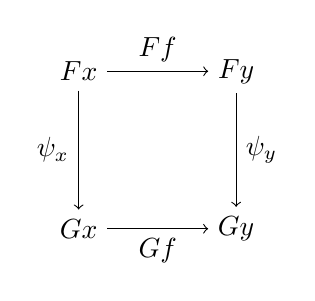
\begin{tikzpicture}
                    \node (FX) at (0, 0) {$Fx$};
                    \node (FY) at(2, 0) {$Fy$};
                    \node (GX) at (0, -2) {$Gx$};
                    \node (GY) at (2, -2) {$Gy$};
                    \draw[->] (FX) -- node[above]{$Ff$} (FY);
                    \draw[->] (GX) -- node[below]{$Gf$} (GY);
                    \draw[->] (FX) -- node[left]{$\psi_x$} (GX);
                    \draw[->] (FY) -- node[right]{$\psi_y$} (GY);
                \end{tikzpicture}
            \end{gather*}
        \end{enumerate}
    }
    \begin{definition}[Functor category]\index{functor!category}
        Consider two categories $\mathbf{C}$ and $\mathbf{D}$, where $\mathbf{C}$ is small. The functors $\func{F}{C}{D}$ form the objects of a category with the natural transformations as morphisms. This category is denoted by $\funccat{C}{D}$ or $\mathbf{D}^\mathbf{C}$ (the latter is a generalization of \cref{set:function_set}).
    \end{definition}

    \newdef{Dinatural transformation}{
        Consider two profunctors $\profunc{F,G}{C}{C}$ or, more generally, two functors $F,G:\mathbf{C}^{\text{op}}\times\mathbf{C}\rightarrow\mathbf{D}$. A dinatural transformation is a family of morphisms \[\eta_x:F(x,x)\rightarrow G(x,x)\] that make Diagram~\ref{fig:dinatural} commute for every morphism $f:y\rightarrow x$.
    }

    \begin{figure}[ht!]
        \centering
        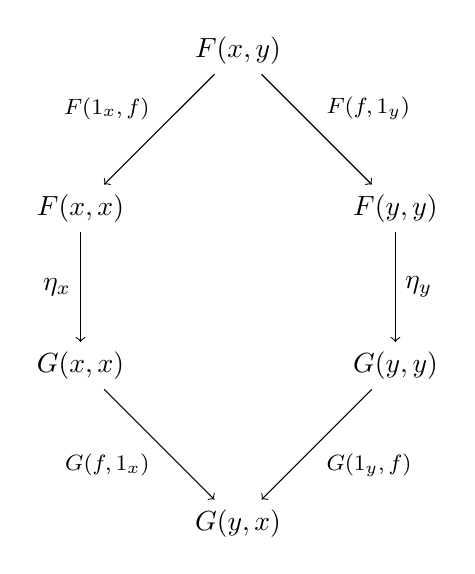
\begin{tikzpicture}
            \node (ab) at (0, 6) {$F(x,y)$};
            \node (F1) at (-2, 4) {$F(x,x)$};
            \node (F2) at (2, 4) {$F(y,y)$};
            \node (G1) at (-2, 2) {$G(x,x)$};
            \node (G2) at (2, 2) {$G(y,y)$};
            \node (ba) at (0, 0) {$G(y,x)$};

            \draw[->] (ab) edge node[above left]{\footnotesize$F(\mathbbm{1}_x,f)$} (F1) (F1) edge node[left]{$\eta_x$} (G1) (G1) edge node[below left]{\footnotesize$G(f,\mathbbm{1}_x)$} (ba);
            \draw[->] (ab) edge node[above right]{\footnotesize$F(f,\mathbbm{1}_y)$} (F2) (F2) edge node[right]{$\eta_y$} (G2) (G2) edge node[below right]{\footnotesize$G(\mathbbm{1}_y,f)$} (ba);
        \end{tikzpicture}
        \caption{Dinatural transformation.}
        \label{fig:dinatural}
    \end{figure}

    \newdef{Representable functor}{\index{representable}\index{representation}
        Let $\mathbf{C}$ be a locally small category. A functor $\func{F}{C}{Set}$ is said to be representable if there exists an object $x\in\ob{C}$ such that $F$ is naturally isomorphic to $h^x$. The pair $(x,\psi:F\Rightarrow h^x)$ is called a \textbf{representation} of $F$.
    }

    \begin{theorem}[Yoneda lemma]\index{Yoneda!lemma}
        Let $\mathbf{C}$ be a locally small category and let $\func{F}{C}{Set}$ be a functor. For every object $x\in\ob{C}$, there exists a natural isomorphism\footnote{Here, the fact that $\mathrm{Nat}(h^-,-)$ can be seen as a functor $\mathbf{Set}^{\mathbf{C}}\times\mathbf{C}\rightarrow\mathbf{Set}$ is used.}
        \begin{gather}
            \eta_x:\mathrm{Nat}(h^x,F)\rightarrow Fx:\psi\mapsto\psi_x(\mathbbm{1}_x)\,.
        \end{gather}
    \end{theorem}

    \begin{result}[Yoneda embedding]\index{Yoneda!embedding}
        When $F$ is another hom-functor $h^y$, the following result is obtained:
        \begin{gather}
            \mathrm{Nat}(h^x,h^y)\cong\mathbf{C}(y,x)\,.
        \end{gather}
        Note that $y$ appears in the first argument on the right-hand side.

        Let $\mathbf{C}(f,-)$ denote the natural transformation corresponding to the morphism $f\in\mathbf{C}(y,x)$. The functor $h^-$, mapping an object $x\in\ob{C}$ to its hom-functor $\mathbf{C}(x,-)$ and a morphism $f\in\mathbf{C}(y,x)$ to the natural transformation $\mathbf{C}(f,-)$, can also be interpreted as a covariant functor $G:\mathbf{C}^{\text{op}}\rightarrow\mathbf{Set}^{\mathbf{C}}$. This way, the Yoneda lemma can be seen to give rise to an embedding $h^-$ of $\mathbf{C}^{\text{op}}$ in the functor category $\mathbf{Set}^{\mathbf{C}}$.

        As usual, all of this can be done for contravariant functors. This gives an embedding
        \begin{gather}
            \mathcal{Y}:=h_-:\mathbf{C}\hookrightarrow\mathbf{Psh(C)}\,,
        \end{gather}
        called the Yoneda embedding.
    \end{result}

    \newdef{Local object}{\index{local!object}\label{cat:local_object}
        Consider a collection of morphisms $S\subseteq\mathrm{hom}(\mathbf{C})$. An object $c\in\ob{C}$ is said to be $S$-local if the Yoneda embedding $\mathcal{Y}c$ maps morphisms in $S$ to isomorphisms in $\mathbf{Set}$. A morphism $f\in\mathrm{hom}(\mathbf{C})$ is said to be $S$-local if its image under the Yoneda embedding of every $S$-local object is an isomorphism in $\mathbf{Set}$.
    }

\subsection{Equivalences}

    \newdef{Equivalence of categories}{\index{equivalence!of categories}
        Two categories $\mathbf{C},\mathbf{D}$ are said to be equivalent if there exist functors $\func{F}{C}{D}$ and $\func{G}{D}{C}$ such that $F\circ G$ and $G\circ F$ are naturally isomorphic to the identity functors.

        A weaker notion is that of a \textbf{weak equivalence}. Two categories $\mathbf{C},\mathbf{D}$ are said to be weakly equivalent if there exist functors $\func{F}{C}{D}$ and $\func{G}{D}{C}$ that are fully faithful and essentially surjective. Assuming the axiom of choice, every weak equivalence is also a (strong) equivalence (in fact this statement is equivalent to the axiom of choice).
    }

    \newdef{Skeletal category}{\index{category!skeletal}
        A category in which every isomorphism is necessarily an identity morphism. The \textbf{skeleton} of a category is an equivalent skeletal category (often taken to be a subcategory by choosing a representative from every isomorphism class).

        If one does not assume the axiom of choice, the skeleton is merely a weakly equivalent skeletal category.
    }

    \newdef{Decategorification}{\index{decategorification}\label{cat:decategorification}
        Let $\mathbf{C}$ be an (essentially) small category. The set of isomorphism classes of $\mathbf{C}$ is called the decategorification of $\mathbf{C}$. This amounts to a functor $\func{\mathrm{Decat}}{Cat}{Set}$.
    }

\subsection{Stuff, structure and property}\index{forgetful}

    To classify properties of objects and the \textit{forgetfulness} of functors, it is interesting to make a distinction between stuff, structure and property. Consider for example a group. This is a set (\textit{stuff}) equipped with a number of operations (\textit{structure}) that obey some relations (\textit{properties}).

    Using these notions one can classify forgetful functors in the following way:
    \begin{itemize}
        \item A functor forgets nothing if it is an equivalence of categories.
        \item A functor forgets at most properties if it is fully faithful.
        \item A functor forgets at most structure if it is faithful.
        \item A functor forgets at most stuff if it is just a functor.
    \end{itemize}

    \todo{COMPLETE (see e.g. nLab or the paper ``Why surplus structure is not superfluous'' by Nicholas Teh et al.)}

\subsection{Adjunctions}\index{adjunction}\label{section:adjunction}

    \newdef{Hom-set adjunction}{
        Let $\func{F}{C}{D}$ and $\func{G}{D}{C}$ be two functors. These functors form a (hom-set) adjunction $F\dashv G$ if the following isomorphism is natural in both $x$ and $y$:
        \begin{gather}
            \Phi_{x,y}:\mathbf{D}(Fx,y)\cong\mathbf{C}(x,Gy)\,.
        \end{gather}
        The functor $F$ (resp.~$G$) is called the left (resp.~right) adjoint and the image of a morphism under either of the natural isomorphisms is called the adjunct of the other morphism.\footnote{The terms `adjunct' and `adjoint' are sometimes used interchangeably (cf.~French versus Latin).}.
    }
    \begin{notation}
        An adjunction $F\dashv G$ between categories $\mathbf{C,D}$ is often denoted by \[\mathbf{D}\adj{F}{G}\mathbf{C}\,.\]
    \end{notation}

    \newdef{Unit-counit adjunction}{\index{triangle!identities}\index{unit}\index{zig-zag|see{triangle identity}}\label{cat:unit_counit_adjunction}
        Let $\func{F}{C}{D}$ and $\func{G}{D}{C}$ be two functors. These functors form a unit-counit adjunction if there exist natural transformations
        \begin{align}
            \varepsilon:F\circ G\Rightarrow\mathbbm{1}_\mathbf{D}\\
            \eta:\mathbbm{1}_\mathbf{C}\Rightarrow G\circ F
        \end{align}
        such that the following compositions are identity morphisms:
        \begin{align}
            F\overset{F\eta}{\longrightarrow}FGF&\overset{\varepsilon F}{\longrightarrow}F\,,\\
            G\overset{\eta G}{\longrightarrow}GFG&\overset{G\varepsilon}{\longrightarrow}G\,.
        \end{align}
        These identities are sometimes called the \textbf{triangle} or \textbf{zig-zag identities} (the latter results from the shape of the associated \textit{string diagram}). The transformations $\eta$ and $\varepsilon$ are called the \textbf{unit} and \textbf{counit}, respectively.
    }

    \begin{property}[Equivalence]
        Every hom-set adjunctions induces a unit-counit adjunction where the counit $\varepsilon_y$ is obtained as the adjunct $\Phi^{-1}_{Gy,y}(\mathbbm{1}_{Gy})$ of the identity morphism on $Gy\in\ob{C}$ and the unit $\eta_x$ is given by the adjunct $\Phi_{c,Fc}(\mathbbm{1}_{Fx})$ of the identity morphism at $Fx\in\ob{D}$.

        Conversely, every unit-counit adjunction induces a hom-set adjunction. The (right) adjunct of a morphism $f:Fx\rightarrow y$ is given by the composition
        \begin{gather}
            \widetilde{f}:=Gf\circ\eta_x:x\rightarrow (G\circ F)x\rightarrow Gy
        \end{gather}
        and the (left) adjunct of a morphism $\widetilde{g}:x\rightarrow Gy$ is given by:
        \begin{gather}
            g:=\varepsilon_y\circ F\tilde{g}:Fx\rightarrow(F\circ G)y\rightarrow y\,.
        \end{gather}
    \end{property}

    \newdef{Reflective subcategory}{\index{reflective!category}\label{cat:reflective_inclusion}
        A full subcategory is said to be reflective (resp.~coreflective) if the inclusion functor admits a left (resp.~right) adjoint.
    }

    \begin{property}[Adjoint equivalence]\index{equivalence!adjoint}
        Any equivalence of categories is part of an adjoint equivalence, i.e.~an adjunction for which the unit and counit morphisms are invertible.
    \end{property}
    \begin{property}\label{cat:adjoint_equivalence}
        Given an adjunction, one obtains an adjoint equivalence by restricting to the full subcategories on which the unit and counit become isomorphisms.
    \end{property}

    Adjunctions can also be defined through a third alternative. This links the definition to universal properties.
    \newdef{Universal morphism}{\index{universal!morphism}\label{cat:universal_morphism}
        Consider a functor $\func{F}{C}{D}$ and an object $d\in\ob{D}$. A universal morphism from $d$ to $F$ is a pair $(c,f:d\rightarrow Fc)$ such that all other morphisms $f':d\rightarrow Fc'$ factor uniquely through $f$ by the image of a morphism in $\mathbf{C}$.
    }
    \newadef{Adjoint functor}{
        A functor $\func{F}{C}{D}$ is a left adjoint if for each object $c\in\ob{C}$ there exists a universal morphism from $F$ to $c$. A functor $\func{G}{C}{D}$ is a right adjoint if for each object $d\in\ob{D}$ there exists a universal morphism from $d$ to $G$.

        The functor to which these functors are adjoint can be recovered as that mapping objects to the object-part of their universal morphism.
    }

\section{General constructions}

    \newdef{Dagger category}{\index{category!dagger}\label{cat:dagger_category}
        A category equipped with a contravariant involutive endofunctor, this functor is often denoted by $\func{\dagger}{C}{C}$, similar to the adjoint operator for Hermitian matrices.
    }
    \begin{remark}\index{unitary}\index{self-adjoint}
        The concept of a dagger structure allows the usual definition of \textbf{unitary} and \textbf{self-adjoint} morphisms, i.e.~morphism satisfying
        \begin{gather}
            f^\dagger = f^{-1}\qquad\text{or}\qquad f^\dagger = f\,.
        \end{gather}
    \end{remark}

    \newdef{Comma category}{\index{category!comma}
        Let $\mathbf{A},\mathbf{B}$ and $\mathbf{C}$ be three categories and let $\func{F}{A}{C}$ and $\func{G}{B}{C}$ be two functors. The comma category $F\downarrow G$ is defined as follows:
        \begin{itemize}
            \item\textbf{Objects}: The triples $(x,y,\gamma)$ where $x\in\ob{A},y\in\ob{B}$ and $\gamma:Fx\rightarrow Gy$.
            \item\textbf{Morphisms}: The morphisms $(x,y,\gamma)\rightarrow(k,l,\sigma)$ are pairs $(f,g)$ with $f:x\rightarrow k\in\mathrm{hom}(\mathbf{A})$ and $g:y\rightarrow l\in\mathrm{hom}(\mathbf{B})$ such that $\sigma\circ Ff = Gg\circ\gamma$.
        \end{itemize}
        Composition of morphisms is defined componentwise.
    }
    \newdef{Arrow category}{\index{category!arrow}\index{walking!arrow}\index{interval!category}\label{cat:arrow_category}
        The comma category of the pair of functors $(\mathbbm{1}_{\mathbf{C}},\mathbbm{1}_{\mathbf{C}})$. This is equivalently the functor category $[\mathbf{2},\mathbf{C}]$, where $\mathbf{2}$ is the \textbf{interval category/walking arrow} $\{0\rightarrow1\}$.
    }
    \newdef{Functorial factorization}{\index{factorization!functorial}\label{cat:functorial_factorization}
        A \textit{section} (see \cref{cat:retract}) of the composition functor \[\func{\circ}{[3,C]}{[2,C]}\,,\] where $\mathbf{3}$ is the poset $\{0\rightarrow1\rightarrow2\}$.
    }

    If $F$ is the identity functor and $\func{G}{1}{C}$ picks out a single object, the notion of a slice category is obtained (by interchanging these choices, one can also define \textbf{coslice categories}).
    \newdef{Slice category}{\index{category!slice}\index{over!category}\label{cat:slice}
        Let $\mathbf{C}$ be a category and consider an object $x\in\ob{C}$. The slice category (or \textbf{overcategory}) $\mathbf{C}_{/x}$ of $\mathbf{C}$ over $x$ is defined as follows:
        \begin{itemize}
            \item\textbf{Objects}: The morphisms in $\mathbf{C}$ with codomain $x$, and
            \item\textbf{Morphisms}: The morphisms $f\rightarrow g$ are morphisms $h$ in $\mathbf{C}$ such that $g\circ h = f$.
        \end{itemize}
        By dualizing one obtains the \textbf{undercategory} of $x$.
    }

\subsection{\difficult{Fibred categories}}\label{section:fibred_categories}

    \newdef{Fibre category}{\index{fibre!category}\label{cat:fibre_category}
        Let $\func{\Pi}{C}{D}$ be a functor. The fibre category (of $\Pi$) over $y\in\ob{D}$ is the subcategory of $\mathbf{C}$ consisting of all objects $x\in\ob{C}$ such that $\Pi x=y$ and all morphisms $f\in\mathrm{hom}(\mathbf{C})$ such that $\Pi f=\mathbbm{1}_y$. It will be denoted by $\mathbf{C}_y$.

        Morphisms in $\mathbf{C}$ that are mapped to a morphism $g$ in $\mathbf{D}$ are called \textbf{$g$-morphisms} and, in particular (using the identification of objects and their identity morphisms), morphisms in $\mathbf{C}_y$ are called \textbf{$y$-morphisms}. Similarly, \textbf{$\mathbf{D}$-categories} are defined as the categories equipped with a (covariant) functor to $\mathbf{D}$. (It is not hard to see that these form a \textit{2-category} under composition of functors that respects the $\mathbf{D}$-category structure.)
    }

    \newdef{Cartesian morphism}{\index{Cartesian!morphism}
        Consider a $\mathbf{D}$-category $\func{\Pi}{C}{D}$. A morphism $f$ in $\mathbf{C}$ is called $\Pi$-Cartesian if every $\Pi f$-morphism factors uniquely through a $y$-morphism, where $y$ is the domain of $\Pi f$.

        There also exists a stronger notion. A \textbf{strongly Cartesian morphism} is a morphism $f\in\mathrm{hom}(\mathbf{C})$ such that for every morphism $\varphi\in\mathrm{hom}(\mathbf{C})$ with the same target and every factorization of $\Pi\varphi$ through $\Pi f$, there exists a unique factorization of $\varphi$ through $f$ that maps to the given factorization of $\Pi\varphi$.

        The following diagram, where the triangles commute, should clarify the above (technical) definitions:
        \begin{gather*}
            \begin{tikzpicture}
                \node (X3) at (0,2) {$\forall x'$};
                \node (X1) at (0,0) {$x_1$};
                \node (X2) at (2,0) {$x_2$};
                \node (arrow) at (4,1) {$\overset{\Pi}{\mapsto}$};
                \node (pX3) at (6,2) {$\Pi x'$};
                \node (pX1) at (6,0) {$\Pi x_1$};
                \node (pX2) at (8,0) {$\Pi x_2$};
                \draw[->] (X1) -- node[below]{$f$} (X2);
                \draw[->, dashed] (X3) -- node[left]{$\exists!g$} (X1);
                \draw[->] (X3) -- node[above right]{$\forall\varphi$} (X2);
                \draw[->] (pX1) -- node[below]{$\Pi f$} (pX2);
                \draw[->] (pX3) -- node[left]{$\forall\nu$} (pX1);
                \draw[->] (pX3) -- node[above right]{$\Pi\varphi$} (pX2);
            \end{tikzpicture}
        \end{gather*}
        The diagram for (weak) Cartesian morphisms is obtained by identifying the objects $\Pi x'$ and $\Pi x_1$, i.e.~by restricting to the case $\nu=\mathbbm{1}_{\Pi x_1}$.

        The Cartesian morphisms are said to be \textbf{inverse images} of their projections under $\Pi$ and the object $x_1$ is called an \textbf{inverse image} of $x_2$ by $\Pi f$. The Cartesian morphisms of a fibre category are exactly the isomorphisms of that category.
    }

    \newdef{Fibred category}{\index{fibred!category}\index{Grothendieck!fibration|see{fibred category}}
        A $\mathbf{D}$-category $\func{\Pi}{C}{D}$ is called a fibred category or \textbf{Grothendieck fibration} if the following conditions are satisfied:
        \begin{enumerate}
            \item For each morphism in $\mathbf{D}$, whose codomain lies in the range of $\Pi$, and each lift of this codomain to $\mathbf{C}$, there exists at least one inverse image with the given codomain (in the weak sense).
            \item The composition of two Cartesian morphisms is again Cartesian (in the weak sense).
        \end{enumerate}
        If one instead works with strongly Cartesian morphisms, the second condition follows from the first one. However, it should be noted that, in a fibred category, a morphism is weakly Cartesian if and only if it is strongly Cartesian.
    }
    \newdef{Cleavage}{\index{cleavage}\index{cloven|see{cleavage}}
        Given a $\mathbf{D}$-category $\func{\Pi}{C}{D}$, a cleavage is the choice of a Cartesian $g$-morphism $f:x\rightarrow y$ for every $y\in\ob{C}$ and morphism $g:d\rightarrow \Pi y$. A $\mathbf{D}$-category equipped with a cleavage is said to be \textbf{cloven}.

        The existence of cleavage is sufficient for a category to be fibred and, conversely (assuming the axiom of choice), every fibred category admits a cleavage.
    }

    The following example can be obtained as a Grothendieck fibration with discrete fibres.
    \begin{example}[Discrete fibration]
        A functor $\func{F}{C}{D}$ such that, for every object $x\in\ob{C}$ and every morphism $f:y\rightarrow Fx$ in $\mathbf{D}$, there exists a unique morphism $g:z\rightarrow x$ in $\mathbf{C}$ such that $Fg=f$.
    \end{example}
    \begin{example}[Groupoidal fibration]
        If every morphism is required to be Cartesian, the notion of a groupoid(al) fibration or a \textbf{category fibred in groupoids} is obtained. The reason for this name is that every fibre is a groupoid. An equivalent definition is that the associated \textit{pseudofunctor} (see the construction below) factors through the embedding $\mathbf{Grpd}\hookrightarrow\mathbf{Cat}$.
    \end{example}

    \begin{property}[\difficult{Grothendieck construction}]\index{Grothendieck!construction}
        Every fibred category $\func{\Pi}{C}{D}$ defines a \textit{pseudofunctor}\footnote{See \cref{cat:pseudofunctor}.} $\cfunc{F}{D}{Cat}$ that sends objects to fibre categories and arrows $f:c\rightarrow c'$ to the pullback functor $f^*:\mathbf{C}_{c'}\rightarrow\mathbf{C}_c$ constructed from a Cartesian lift of $f$. This pullback functor acts as follows:
        \begin{itemize}
            \item For every object $x\in\mathbf{C}_{c'}$, $f^*x$ is the domain of the Cartesian lift of $f$ through $x$.
            \item For every morphism $(\alpha:x\rightarrow y)\in\mathbf{C}_{c'}$ there exists a diagram of the form
                \begin{gather*}
                    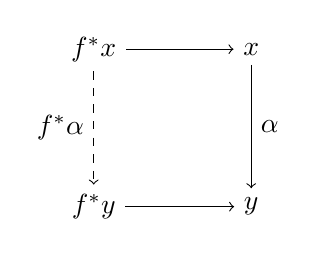
\begin{tikzpicture}
                        \node (fx) at (0, 0) {$f^*x$};
                        \node (x) at (2, 0) {$x$};
                        \node (y) at (2, -2) {$y$};
                        \node (fy) at (0, -2) {$f^*y$};
                        \draw[->] (fx) -- (x);
                        \draw[->] (fy) -- (y);
                        \draw[->] (x) -- node[right]{$\alpha$} (y);
                        \draw[dashed, ->] (fx) -- node[left]{$f^*\alpha$} (fy);
                    \end{tikzpicture}
                \end{gather*}
                Because the horizontal morphism are both projected to $f$ and $\alpha$ is projected to the identity, there exists a unique factorization of the diagram through a morphism $f^*\alpha:f^*x\rightarrow f^*y$.
        \end{itemize}

        Conversely, every \textit{pseudofunctor} gives rise to a fibred category through the Grothendieck construction $\int:\cfunccat{C}{Cat}\rightarrow\mathbf{Cat}/\mathbf{C}$ as follows. (These two constructions constitute a 2-equivalence of 2-categories.). Consider a \textit{pseudofunctor} $\cfunc{F}{C}{Cat}$. The `bundle' $\int\!F$ consists of the following data:
        \begin{itemize}
            \item The objects are pairs $(x,y)$ with $x\in\ob{C}$ and $y\in\mathrm{ob}(Fx)$.
            \item The morphisms $(x,y)\rightarrow(x',y')$ are pairs $\bigl(f:x\rightarrow x',\alpha:y\rightarrow Ff(y')\bigr)$.
        \end{itemize}
        Given a cleavage, the morphisms of the Grothendieck construction are exactly the factorizations of $f$-morphisms through the canonical lifting of $f$ in the cleavage.
    \end{property}
    \begin{property}[Functors]\index{split!cleavage}
        A \textit{pseudofunctor} is a functor if and only if the cleavage of the associated fibred category is \textbf{split(ting)}, i.e.~it contains all identities and is closed under composition.
    \end{property}

    \newdef{Category of elements}{\index{category!of elements}\label{cat:category_of_elements}
        Consider a presheaf $\cfunc{F}{C}{Set}$. Its category of elements $\mathrm{El}(F)$ or $\int_\mathbf{C}F$ is defined as the comma category $(\mathcal{Y}\downarrow\ !_F)$, where $!_F:\ast\rightarrow\cfunccat{C}{Set}$ sends the unique object to $F$ itself. Equivalently, it is the category with objects the pairs $(c,x)\in\ob{C}\times Fc$ and morphisms $f\in\mathbf{C}(c,c')$ such that $c = Ff(c')$, i.e.~it is the Grothendieck construction applied to $F$.

        This category comes equipped with a canonical forgetful functor
        \begin{gather}
            \mathbf{C}_F:\mathrm{El}(F)\rightarrow\mathbf{C}:(c,x)\mapsto c\,.
        \end{gather}
    }
    \remark{The category of elements is often defined for covariant functors. To obtain that definition, one should take the opposite of the category of elements (and also take the opposite of the forgetful functor).}

\subsection{Monads}

    \newdef{Monad}{\index{monad}\label{cat:monad}
        A monad is a triple $(T,\mu,\eta)$ where $\func{T}{C}{C}$ is an endofunctor and $\mu:T^2\rightarrow T, \eta:\mathbbm{1}_{\mathbf{C}}\rightarrow T$ are natural transformations satisfying the following (coherence) conditions:
        \begin{enumerate}
            \item As natural transformations from $T^3$ to $T$:
            \begin{gather}
                \mu\circ T\mu = \mu\circ\mu_T\,.
            \end{gather}
            \item As natural transformations from $T$ to itself:
            \begin{gather}
                \mu\circ T\eta = \mu\circ\eta_T = \mathbbm{1}\,.
            \end{gather}
        \end{enumerate}
        These conditions say that a monad is a monoid (\cref{algebra:monoid}) in the category $\mathbf{End}_{\mathbf{C}}$ of endofunctors on $\mathbf{C}$. Accordingly, $\eta$ and $\mu$ are often called the \textbf{unit} and \textbf{multiplication} maps.
    }

    \begin{example}[Adjunction]\label{cat:monad_from_adjunction}
        Every adjunction $F\dashv G$, with unit $\varepsilon$ and counit $\eta$, induces a monad of the form $(GF,G\varepsilon F,\eta)$.
    \end{example}

    \newdef{Algebra over a monad\footnotemark}{\index{algebra!over a monad}\index{module}\index{carrier}\label{cat:algebra_monad}
        \footnotetext{A more suitable name would be ``module over a monad'', since these are modules over a monoid if monads are regarded as monoids in $\mathbf{End}_\mathbf{C}$.}
        Consider a monad $(T,\mu,\eta)$ on a category $\mathbf{C}$. An algebra over $T$ or $T$-algebra is a couple $(x,\kappa)$, where $x\in\ob{C}$ and $\kappa:Tx\rightarrow x$, such that the following conditions are satisfied:
        \begin{enumerate}
            \item $\kappa\circ T\kappa = \kappa\circ\mu_x$, and
            \item $\kappa\circ\eta_x = \mathbbm{1}_x$.
        \end{enumerate}
        Morphisms $(x,\kappa_x)\rightarrow(y,\kappa_y)$ of $T$-algebras are morphisms $f:x\rightarrow y$ in $\mathbf{C}$ such that $f\circ\kappa_x = \kappa_y\circ Tf$. An algebra of the form $(Tx,\mu_x)$ is said to be \textbf{free}. The object $x$ is called the \textbf{carrier} of the algebra
    }
    \newdef{Eilenberg--Moore category}{\index{Eilenberg--Moore category}\label{cat:eilenberg_moore}
        Given a monad $T$ over a category $\mathbf{C}$, the Eilenberg--Moore category $\mathbf{C}^T$ is defined as the category of $T$-algebras.
    }
    \newdef{Kleisli category}{\index{Kleisli category}\label{cat:kleisli_category}
        Consider a monad $T$ on a category $\mathbf{C}$. The Kleisli category $\mathbf{C}_T$ is defined as the full subcategory of $\mathbf{C}^T$ on the free $T$-algebras. This is equivalently the category with objects $\mathrm{ob}(\mathbf{C}_T):=\ob{C}$ and morphisms $\mathbf{C}_T(x,y):=\mathbf{C}(x,Ty)$.

        Morphisms in the Kleisly category are composed in the `obvious way':
        \begin{gather}
            f\circ_{\mathbf{C}_T} g := \mu_Z\circ Tf\circ g
        \end{gather}
        for all $f\in\mathbf{C}_T(Y,TZ)$ and $g\in\mathbf{C}_T(X,TY)$.
    }

    \newdef{Monadic adjunction}{\index{adjunction!monadic}
        Consider an adjunction $L\dashv R$ between categories $\mathbf{C}$ and $\mathbf{D}$ with the induced monad $T$. The natural morphism $R\varepsilon:T\circ R\Rightarrow R$ endows $R$ with a $T$-algebra structure and, hence, induces a functor $\mathbf{C}\rightarrow\mathbf{D}^T$ between $\mathbf{C}$ and the Eilenberg-Moore category of $T$. $L\dashv R$ is said to be monadic if this functor is an equivalence.
    }
    \newdef{Monadic functor}{\index{functor!monadic}
        A functor is said to be monadic if it admits a left adjoint such that the adjunction is monadic.
    }

    The converse of \ref{cat:monad_from_adjunction} is also true:
    \begin{property}
        Every monad $\func{T}{C}{C}$ can be obtained from an adjunction. The canonical choice is the adjunction
        \begin{gather}
            \mathbf{C}\adj{F_T}{U_T}\mathbf{C}^T\,,
        \end{gather}
        where $F_T$ is the forgetful functor and $U_T$ sends an object to the free $T$-algebra on it.
    \end{property}

    The following theorem characterizes monadic functors (for more information on some of the concepts, see \cref{section:morphisms} further below).
    \begin{theorem}[Beck's monadicity theorem]\index{Beck's monadicity theorem}
        Consider a functor $\func{F}{C}{D}$. This functor is monadic if and only if the following conditions are satisfied:
        \begin{itemize}
            \item $F$ admits a left adjoint.
            \item $F$ reflects isomorphisms.
            \item $\mathbf{C}$ has all coequalizers of $F$-split parallel pairs\footnote{These are parallel pairs $f,g$ such that the images $Ff,Fg$ under $F$ admit a split coequalizer.} and $F$ preserves these coequalizers.
        \end{itemize}
    \end{theorem}
    \begin{remark}[Crude monadicity theorem]
        A sufficient condition for monadicity is obtained by replacing the third condition above by the following weaker statement: ``$\mathbf{C}$ has all coequalizers of reflexive pairs and $F$ preserves these coequalizers.''
    \end{remark}

    \newdef{Closure operator}{\index{closure!operator}\index{modal!operator|seealso{closure operator}}\index{modal!type}\label{cat:closure_operator}
        Consider a monad $(\func{T}{C}{C},\eta,\mu)$. This monad is called a closure operator or \textbf{modal operator} if the multiplication map is a natural isomorphism, i.e.~if the monad is idempotent. Equivalently, it is idempotent if and only if $\eta\circ T$ is a natural isomorphism.

        Given a closure operator $\func{T}{C}{C}$, the object $Tx$ is called the closure of $x\in\ob{C}$ and the associated morphism $\eta_x$ is called the \textbf{closing map}. An object $x\in\ob{C}$ itself is said to be $T$\textbf{-closed} exactly if its closing map is an isomorphism.

        An object $x\in\ob{C}$ is called a \textbf{modal type} if the unit $\eta_x:x\rightarrow Tx$ is an isomorphism.
    }
    \begin{property}
        Every (co)reflective subcategory inclusion (\cref{cat:reflective_inclusion}) induces a closure operator. Conversely, every closure operator is induced by a (co)reflective subcategory.
    \end{property}

    \begin{remark}[\difficult{Bicategories}]
        A monad can be defined in any bicategory as a 1-morphism $t:x\rightarrow x$ together with two 2-morphisms that satisfy conditions similar to the ones above. The above definition is then just a specific case of this more general definition in $\mathbf{Cat}$.

        In the general setting one can then also define a \textbf{module} over a monad. First of all, one can regard any object $x\in\ob{C}$ as a functor from the terminal category $\mathbf{1}$. By replacing $\mathbf{1}$ by any other category in the ordinary definition one obtains a general algebra (or module). It is this definition that readily generalizes to bicategories, i.e.~a module is a 1-morphism $a:x\rightarrow y$ together with a 2-morphism that satisfies the same conditions as an algebra over a monad in $\mathbf{Cat}$.
    \end{remark}

\section{Morphisms and diagrams}\label{section:morphisms}
\subsection{Morphisms}

    \newdef{Section}{\index{section}\index{retract}\label{cat:retract}
        A section of a morphism $f:x\rightarrow y$ is a right inverse, i.e.~a morphism $g:y\rightarrow x$ such that $f\circ g=\mathbbm{1}_y$. $f$ itself is called a \textbf{retraction} of $g$ and $y$ is called a \textbf{retract} of $x$.
    }

    \newdef{Monomorphism}{\index{monomorphism}
        Let $\mathbf{C}$ be a category. A morphism $\mu\in\mathbf{C}(x,y)$ is called a monomorphism, \textbf{mono} or \textbf{monic morphism} if for every object $z\in\ob{C}$ and every two morphisms $\alpha_1,\alpha_2\in\mathbf{C}(z,x)$ such that $\mu\circ\alpha_1 = \mu\circ\alpha_2$, one can conclude that $\alpha_1=\alpha_2$.
    }
    \newdef{Epimorphism}{\index{epimorphism}
        Let $\mathbf{C}$ be a category. A morphism $\varepsilon\in\mathbf{C}(x,y)$ is called an epimorphism, \textbf{epi} or \textbf{epic morphism} if for every object $z\in\ob{C}$ and every two morphisms $\alpha_1,\alpha_2\in\mathbf{C}(y,z)$ such that $\alpha_1\circ\varepsilon = \alpha_2\circ\varepsilon$, one can conclude that $\alpha_1=\alpha_2$.

        A family of morphisms $\{f_i:x_i\rightarrow y\}_{i\in I}$ is called \textbf{jointly epimorphic} if
        \begin{gather}
            \alpha_1\circ f_i = \alpha_2\circ f_i
        \end{gather}
        for all $i\in I$ implies that $\alpha_1=\alpha_2$.
    }

    \newdef{Split monomorphism}{\index{split!morphism}
        A morphism $f:x\rightarrow y$ that is a section of some other morphism $g:y\rightarrow x$. It can be shown that every split mono is in fact a mono and even an \textbf{absolute mono}, i.e.~it is preserved by all functors.

        The morphism $g$ can be seen to satisfy the dual condition and, hence, is called a \textbf{split epimorphism}. It can be shown to be an absolute epi.
    }

    \newdef{Balanced category}{\index{category!balanced}\label{cat:balanced}
        A category in which every monic epi is an isomorphism.
    }

    \newdef{Reflexive pair}{
        Two parallel morphisms $f,g:x\rightarrow y$ are said to form a reflexive pair if they have a common section, i.e.~if there exists a morphism $\sigma:y\rightarrow x$ such that $f\circ\sigma=g\circ\sigma=\mathbbm{1}_y$.
    }

    \newdef{Subobject}{\index{subobject}
        Let $\mathbf{C}$ be a category and let $x\in\ob{C}$ be any object. A subobject $y$ of $x$ is a mono $y\hookrightarrow x$.

        In fact, one should work up to isomorphisms and, accordingly, the formal definition goes as follows: a subobject $y$ of $x$ is an isomorphism class of monos $i:y\hookrightarrow x$ in the slice category $\mathbf{C}_{/x}$.
    }
    \newdef{Well-powered category}{\index{well-!powered}
        A category $\mathbf{C}$ such that for every object $x\in\ob{C}$ the class of subobjects $\mathrm{Sub}(x)$ is small.
    }

\subsection{Initial and terminal objects}

    \newdef{Initial object}{\index{initial}
        An object $\emptyset$ such that for every other object $x$ there exists a unique morphism $\iota_x:\emptyset\rightarrow x$. If one drops the uniqueness, the notion of a \textbf{weakly initial object} is obtained.
    }
    \newdef{Terminal object}{\index{terminal}
        An object $1$ such that for every other object $x$ there exists a unique morphism $\tau_x:x\rightarrow 1$.
    }
    \begin{property}[Uniqueness]
        If an initial (or terminal) object exists, it is unique (up to isomorphisms).
    \end{property}

    \newdef{Zero object}{\index{zero!object}\label{cat:zero_object}
        An object that is both initial and terminal. The zero object is often denoted by $0$.
    }
    \begin{property}[Zero morphism]
        From the definition of the zero object it follows that for any two objects $x,y$ there exists a unique morphism $0_{xy}:x\rightarrow0\rightarrow y$.
    \end{property}
    \newdef{Pointed category}{\index{pointed!category}\label{cat:pointed_category}
        A category containing a zero object.
    }

    \newdef{Global element}{\index{global!element}\label{cat:global_element}
        Let $\mathbf{C}$ be a category with a terminal object $1$. A global element of an object $x\in\ob{C}$ is a morphism $1\rightarrow x$.
    }
    \begin{property}
        Every global element is monic.
    \end{property}

    \newdef{Pointed object}{\index{pointed!object}\label{cat:pointed_object}
        An object $x$ equipped with a global element $1\rightarrow x$. This morphism is sometimes called the \textbf{basepoint}.
    }

    \begin{remark}\label{cat:global_elements_remark}
        In the category $\mathbf{Set}$, the elements of a set $S$ are in one-to-one correspondence with the global elements of $S$. Furthermore, there is the the important property (\textit{axiom of functional extensionality}) that two functions $f,g:S\rightarrow S'$ coincide if their values at every element $s\in S$ coincide or, equivalently, if their precompositions with global elements coincide.

        However, this way of checking equality can fail in other categories. Consider for example $\mathbf{Grp}$, the category of groups, with its zero object $0=\{e\}$. The only morphism from this group to any other group $G$ is the one mapping $e$ to the unit in $G$. It is obvious that precomposition with this morphism says nothing about the equality of other morphisms. To recover the extensionality property from $\mathbf{Set}$, the notion of an `element' should be generalized:
    \end{remark}
    \newdef{Generalized element}{\index{shape}
        Let $\mathbf{C}$ be a category and consider an object $x\in\ob{C}$. For any object $y\in\ob{C}$, a morphism $y\rightarrow x$ is called a generalized element of $x$. These morphisms are also called \textbf{$y$-elements} in $x$ or elements of \textbf{shape} $y$ in $x$.
    }

    \newdef{Generator}{\index{generator}\index{separator|see{generator}}\label{cat:generator}
        Let $\mathbf{C}$ be a category. A collection of objects $\mathcal{O}\subset\ob{C}$ is called a collection of generators or \textbf{separators} for $\mathbf{C}$ if the generalized elements of shape $\mathcal{O}$ are sufficient to distinguish between all morphisms in $\mathbf{C}$:
        \begin{gather}
            \forall x,y\in\ob{C}:\forall f,g\in\mathbf{C}(x,y):\bigl(f\neq g\implies\exists o\in\mathcal{O}:\exists h\in\mathbf{C}(o,x): f\circ h\neq g\circ h\bigr)\,.
        \end{gather}
    }
    \newdef{Well-pointed category}{\index{well-!pointed}
        A category for which the terminal object is a generator.
    }

    \newdef{Free object}{\index{free}
        Consider a forgetful functor $\func{U}{C}{D}$ (whatever this may mean). An object $c\in\ob{C}$ is said to be free over an object $x\in\ob{D}$ if there exists a universal morphism $\eta_x:x\rightarrow Uc$. These are the initial objects of the comma categories $x/\mathbf{U}$.
    }
    \begin{property}[Free functor]\index{free!functor}
        Note that if the forgetful functor admits a left adjoint $\func{F}{D}{C}$, every object in the image of $F$ is free according to the previous definition. Moreover, if $U$ admits a free object for every $x\in\ob{D}$, it has a left adjoint. For this reason, left adjoints to fortgetful functors are often called free functors.
    \end{property}

    \Cref{cat:algebra_monad} can be generalized to endofunctors as follows:
    \newdef{Algebra over an endofunctor}{\index{carrier}\label{cat:endofunctor_algebra}
        Consider an endofunctor $\func{F}{C}{C}$. An algebra over $F$ is a pair $(x,f:Fx\rightarrow x)$, where $x\in\ob{C}$ is often called the \textbf{carrier}.
    }
    \begin{property}\label{cat:algebraically_free_monad}
        The category of algebras over an endofunctor is equivalent to the Eilenberg--Moore category of the \textbf{(algebraically-)free monad} it generates (if it exists).
    \end{property}
    \begin{construct}
        This property could actually be interpreted as the definition of the free monad generated by an endofunctor. If it exists, it can be obtained as the monad induced by the free-forgetful adjunction induced by $F\mathbf{Alg}\rightarrow\mathbf{C}$.

        When the free functor exists, it can be constructed as follows. Consider an endofunctor $\func{F}{C}{C}$. The term introduction of an inductive type corresponds to a morphism $Fc\rightarrow c$, i.e.~to an algebra over $F$. Now, algebras over $F$ should correspond to the algebras over its free monad, the functor $F^*:=U\circ\mathcal{F}$, where $U:F\mathbf{Alg}\rightarrow\mathbf{C}$ is the forgetful functor and $\mathcal{F}:\mathbf{C}\rightarrow F\mathbf{Alg}$ the free functor. The latter sends every object $d\in\ob{C}$ to the initial object of the comma category $d/U$, i.e.~to an object $(c,\alpha: Fc\rightarrow c,\beta:d\rightarrow c)$. However, as long as $\mathbf{C}$ admits coproducts, such a triple is equivalent to a pair $(c,\gamma:d+Fc\rightarrow c)$. Since the latter is an algebra over $\mathbbm{1}_\mathbf{C}+F$, one finds that algebras over $F$ are equivalent to initial algebras over $\mathbbm{1}_\mathbf{C}+F$.
    \end{construct}

    \begin{theorem}[Lambek]
        If $\func{F}{C}{C}$ has an initial algebra $f:Fx\rightarrow x$, then $f$ is an isomorphism.
    \end{theorem}

\subsection{Lifts}

    \newdef{Lifts and extensions}{\index{lift}\index{extension}
        A lift of a morphism $f:x\rightarrow y$ along an epi $e:z\rightarrow y$ is a morphism $g:x\rightarrow z$ satisfying $f=e\circ g$. Dualizing this definition gives the notion of extensions. (The epi/mono condition is often dropped in the literature.)
    }
    \newdef{Lifting property}{\index{orthogonal!lifting}\label{cat:lifting_property}
        A morphism $f:x\rightarrow y$ has the left lifting property with respect to a morphism $g:x'\rightarrow y'$ (or $g$ has the right lifting property with respect to $f$) if for every commutative diagram
        \begin{gather*}
            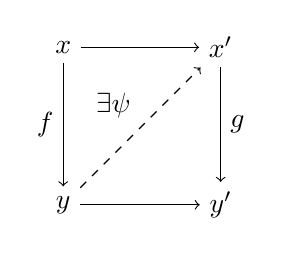
\begin{tikzpicture}
                \node (A) at (0, 0) {$x$};
                \node (B) at (0, -2) {$y$};
                \node (C) at (2, 0) {$x'$};
                \node (D) at (2, -2) {$y'$};
                \draw[->] (A) -- node[left]{$f$} (B);
                \draw[->] (A) -- (C);
                \draw[->, dashed] (B) -- node[above left]{$\exists\psi$} (C);
                \draw[->] (B) -- (D);
                \draw[->] (C) -- node[right]{$g$} (D);
            \end{tikzpicture}
        \end{gather*}
        there exists a morphism $\psi:y\rightarrow x'$ such that the triangles commute. If the morphism $\psi$ is unique, then $f$ and $g$ are said to be \textbf{orthogonal}.
    }
    \newdef{Injective / projective morphisms}{\index{injective!morphism}\index{projective!morphism}
        Consider a class of morphisms $I\subseteq\mathrm{hom}(\mathbf{C})$. A morphism $f\in\mathrm{hom}(\mathbf{C})$ is said to be $I$-injective (resp.~$I$-projective) if it has the right (resp.~left) lifting property with respect to all morphisms in $I$.

        Given a set of morphisms $I$, the sets of $I$-injective and $I$-projective morphisms are denoted by $\mathrm{rlp}(I)$ and $\mathrm{llp}(I)$, respectively.
    }
    \newdef{Injective and projective objects}{\index{injective!object}\index{projective!object}
        If $\mathbf{C}$ has a terminal object $1$, an object $x$ is called $I$-injective if its terminal morphism is $I$-injective. If $\mathbf{C}$ has an initial object, $I$-projective objects can be defined dually. (See \cref{fig:inj_proj}.)

        \begin{figure}[ht!]
            \centering
            \begin{subfigure}[b]{0.49\textwidth}
                \centering
                \begin{tikzpicture}
                    \node (X) at (0, 0) {$x$};
                    \node (Y) at (0, -2) {$y$};
                    \node (C) at (2, 0) {$i$};
                    \draw[->] (X) -- node[left]{$\forall f\in I$} (Y);
                    \draw[->] (X) -- node[above]{$g$} (C);
                    \draw[dashed, ->] (Y) -- node[below right]{$\exists\psi$} (C);
                \end{tikzpicture}
                \caption{Injective object $i$.}
                \label{fig:injective_object}
            \end{subfigure}
            \begin{subfigure}[b]{0.49\textwidth}
                \centering
                \begin{tikzpicture}
                    \node (X) at (2, 2) {$x$};
                    \node (Y) at (2, 0) {$y$};
                    \node (C) at (0, 0) {$p$};
                    \draw[->] (X) -- node[right]{$\forall f\in I$} (Y);
                    \draw[->] (C) -- node[below]{$g$} (Y);
                    \draw[dashed, ->] (C) -- node[above left]{$\exists\psi$} (X);
                \end{tikzpicture}
                \caption{Projective object $p$.}
                \label{fig:projective_object}
            \end{subfigure}
            \caption{Injective and projective objects.}
            \label{fig:inj_proj}
        \end{figure}
        If $I$ is the class of monomorphisms (resp.~epimorphisms), the terminology is simplified to \textbf{injective} (resp.~\textbf{projective}) objects. For projective objects, this is also equivalent to requiring that the (covariant) hom-functor preserves epimorphisms.

        A category $\mathbf{C}$ is said to \textbf{have enough injectives} if, for every object, there exists a monomorphism into an injective object. The category is said to \textbf{have enough projectives} if, for every object, there exists an epimorphism from a projective object.
    }
    \newdef{Fibrations and cofibrations}{\index{fibration}
        Consider a category $\mathbf{C}$ together with a class $I\subseteq\mathrm{hom}(\mathbf{C})$ of morphisms. A morphism $f\in\mathrm{hom}(\mathbf{C})$ is called an $I$-fibration (resp. $I$-cofibration) if it has the right (resp.~left) lifting property with respect to all $I$-projective (resp.~$I$-injective) morphisms.
    }

\subsection{Limits and colimits}\label{section:diagrams}

    \newdef{Diagram}{\index{diagram}
        A diagram in $\mathbf{C}$ with index category $\mathbf{I}$ is a (covariant) functor $\func{D}{I}{C}$.
    }

    \newdef{Cone}{\index{cone}
        Let $\func{D}{I}{C}$ be a diagram. A cone from $c\in\ob{C}$ to $D$ consists of a family of morphisms $\psi_i:c\rightarrow Di$ indexed by $\mathbf{I}$ such that $\psi_j = Df\circ\psi_i$ for all morphisms $f:i\rightarrow j\in\mathrm{hom}(\mathbf{I})$. (This is depicted in \cref{fig:cone_component}.)

        \begin{figure}[ht!]
            \centering
            \begin{subfigure}[b]{0.49\textwidth}
                \centering
                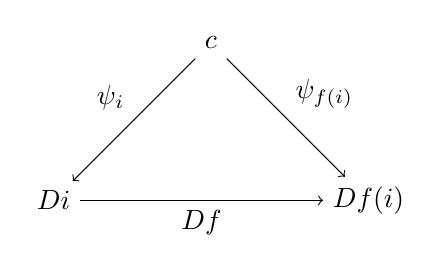
\begin{tikzpicture}
                    \node (1) at (0, 0) {$c$};
                    \node (2) at (-2, -2) {$Di$};
                    \node (3) at (2, -2) {$Df(i)$};
                    \draw[->] (1) -- node[above left]{$\psi_i$} (2);
                    \draw[->] (1) -- node[above right]{$\psi_{f(i)}$} (3);
                    \draw[->] (2) -- node[below]{$Df$} (3);
                \end{tikzpicture}
                \caption{Component of cone over $D$.}
                \label{fig:cone_component}
            \end{subfigure}
            \begin{subfigure}[b]{0.49\textwidth}
                \centering
                \begin{tikzpicture}
                    \node (1) at (0, -2) {$Di$};
                    \node (2) at (-2, 0) {$a$};
                    \node (3) at (2, 0) {$b$};
                    \draw[<-] (1) -- node[below left]{$\psi_i$} (2);
                    \draw[<-] (1) -- node[below right]{$\phi_i$} (3);
                    \draw[->] (2) -- node[above]{$f$} (3);
                \end{tikzpicture}
                \caption{Morphism of cones.}
                \label{fig:cone_morphism}
            \end{subfigure}
            \caption{Category of cones.}
            \label{fig:cone}
        \end{figure}
    }
    \begin{adefinition}\index{diagonal!functor}
        The above definition can be reformulated by defining an additional functor $\Delta_x:\mathbf{I}\rightarrow\mathbf{C}$ that maps every element $i\in\ob{I}$ to $x$ and every morphism $g\in\mathrm{hom}(\mathbf{I})$ to $\mathbbm{1}_x$, i.e.~$\Delta:C\rightarrow[\mathbf{I},\mathbf{C}]$ is the \textbf{diagonal functor}. The morphisms $\psi_i$ can then be seen to be the components of a natural transformation $\psi:\Delta_x\Rightarrow D$. Hence, a cone $(x,\psi)$ is an element of $[\mathbf{I},\mathbf{C}](\Delta_x,D)$.
    \end{adefinition}
    \newdef{Morphism of cones}{\index{morphism!of cones}
        Let $\func{D}{I}{C}$ be a diagram and let $(x,\psi)$ and $(y,\phi)$ be two cones over $D$. A morphism between these cones is a morphism of the apexes $f:x\rightarrow y$ such that the diagrams of the form \ref{fig:cone_morphism} commute for all $i\in\ob{I}$. The cones over $D$ together with these morphisms form a category $\mathbf{Cone}(D)$. In fact this can easily be seen to be the comma category $\Delta\downarrow D$.
    }

    \newdef{Limit}{\index{limit}\label{cat:limit}
        Consider a diagram $\func{D}{I}{C}$. The limit of this diagram, denoted by $\lim D$, is (if it exists) the terminal object of the category $\mathbf{Cone}(D)$.
    }
    \begin{remark}\index{projective!limit}\index{inductive!limit}\label{cat:projective_remark}
        In the older literature, the name \textbf{projective limit} was sometimes used. The dual notion, a \textbf{colimit}, was often called an \textbf{inductive limit} in the older literature.
    \end{remark}

    This definition leads to the following universal property.
    \begin{uproperty}\label{cat:limit_uproperty}
        Let $\func{D}{I}{C}$ be a diagram. For every cone $(x,\psi)\in\mathbf{Cone}(D)$, there exists a unique morphism $f:x\rightarrow\lim D$. This defines a bijection
        \begin{gather}
            \funccat{I}{C}(\Delta_x,D)\cong\mathbf{C}(x,\lim D)\,.
        \end{gather}
        If all (small) limits exist, the limit functor $\func{\lim}{[I,C]}{C}$ can be defined. The universal property of limits then implies that it is right adjoint to the constant functor $\Delta$.

        For diagrams in $\mathbf{Set}$, one can use the fully faithfulness of the Yoneda embedding to obtain the following expression:
        \begin{gather}
            \lim D\cong\funccat{I}{Set}(\Delta_\ast,D)\,.
        \end{gather}
    \end{uproperty}
    \begin{remark}
        In \cref{section:enriched_category_theory} on enriched category theory, a generalization of the above construction (the so-called \textit{weighted limits}) will be given that is better suited to the enriched setting and allows to express a wide variety of constructions as (weighted) limits.
    \end{remark}

    \begin{example}[Terminal object]
        The terminal object $1$ is the limit of the empty diagram.
    \end{example}

    \newdef{Finitely complete category}{\index{category!complete}
        A category is said to be finitely complete if it has all finite limits. If all (small) limits exist, the category is said to be \textbf{complete}. The dual notion for colimits is called \textbf{(finite) cocompleteness}.
    }
    \begin{example}[Presheaf categories]\label{cat:complete_presheaf_category}
        All presheaf categories are both complete and cocomplete.
    \end{example}

    \newdef{Continuous functor}{\index{continuity!functor}\label{cat:continuity}
        A functor that preserves all small limits.
    }
    A more restricted form is also common in the literature.
    \newdef{Exact functor}{\index{exact!functor}\label{cat:exact_functor}
        A functor that preserves all finite limits is said to be \textbf{left exact}. Analogously, a functor that preserves all finite colimits is said to be \textbf{right exact}.
    }

    \begin{example}[Hom-functors]
        In a locally small category every hom-functor is continuous (in fact these functors even preserve limits that are not necessarily small). This implies for example that
        \begin{gather}
            \mathbf{C}(x,\lim D)\cong\lim\mathbf{C}(x,D)\,.
        \end{gather}
    \end{example}

    In the case where $\mathbf{C}$ is small, one can characterize the Yoneda embedding through a universal property:
    \begin{uproperty}[Free cocompletion]\index{co-!completion}\label{cat:free_cocompletion}
        The Yoneda embedding $\mathbf{C}\hookrightarrow\widehat{\mathbf{C}}$ turns the presheaf category $\widehat{\mathbf{C}}$ into the \textbf{free cocompletion} of $\mathbf{C}$, i.e.~there exists an equivalence of categories between the functor category of cocontinuous functors $[\widehat{\mathbf{C}},\mathbf{D}]_\mathrm{cont}$ and the ordinary functor category $[\mathbf{C},\mathbf{D}]$.
    \end{uproperty}

    \newdef{Tiny object}{\index{tiny}\label{cat:tiny}
        An object in a locally small category for which the covariant hom-functor preserves small colimits. This is sometimes called a \textbf{small-projective} object since it is in particular projective\footnote{Epimorphisms are characterized by a \textit{pushout} (see \cref{cat:pushout_epi} further below).}.
    }
    \newdef{Cauchy completion}{\index{Cauchy!completion}\index{Karoubi!envelope}
        Let $\mathbf{C}$ be a small category. An important (small and full) subcategory of the free cocompletion of $\mathbf{C}$ is given by the Cauchy completion, i.e.~the subcategory of $\widehat{\mathbf{C}}$ on the tiny objects.\footnote{A generalization in the context of enriched categories is given by the \textit{Karoubi envelope}.} It can be shown that the free cocompletion of the Cauchy completion coincides with the one on $\mathbf{C}$ (up to equivalence).

        A category is said to be \textbf{Cauchy-complete} if it is equivalent to its Cauchy completion. It can be shown that a category is Cauchy-complete if and only if it has all small absolute colimits.
    }

    \newdef{Filtered category}{\index{category!filtered}\label{cat:filtered}
        A category in which every finite diagram admits a cocone. For regular cardinals $\kappa$, this notion can be generalized. A category is said to be $\kappa$-filtered if every diagram with less than $\kappa$ arrows admits a cocone. (In this terminology, filtered categories are the same as $\omega$-filtered categories.)
    }

    \newdef{Directed limit}{\index{limit!directed}
        Consider a diagram $\func{D}{I}{C}$. The limit (resp.~colimit) of $D$ is said to be (co)directed (resp.~directed) if $\mathbf{I}$ is a downward (resp.~upward) directed set \ref{set:directed_set}.
    }
    The following definition is a categorification of the previous one.
    \newdef{Filtered limit}{\index{limit!filtered}
        Consider a diagram $\func{D}{I}{C}$. The limit (resp.~colimit) of $D$ is said to be (co)filtered (resp.~filtered) if $\mathbf{I}$ is a cofiltered (resp.~filtered) category.
    }
    \begin{property}\label{cat:directed_filtered}
        A category has all directed limits if and only if it has all filtered limits. (A dual statement holds for colimits.)
    \end{property}

    \newdef{Finitary functor}{\index{functor!finitary}\label{cat:finitary_functor}
        A functor that preserves all filtered colimits.
    }

    \newdef{Pro-object}{\index{pro-!object}\label{cat:pro_object}
        A functor $\func{F}{I}{C}$ from a cofiltered category. By composing these functors with the Yoneda embedding $\func{\mathcal{Y}}{C}{\cfunccat{C}{Set}}$, pro-objects can also be identified with cofiltered limits of representable presheaves. In conjunction with \cref{cat:projective_remark}, this clarifies the terminology.
    }
    \begin{uproperty}\index{pro-!category}\label{cat:pro_object_uproperty}
        The \textbf{procategory} $\mathbf{Pro(C)}$ is the universal completion of $\mathbf{C}$ under cofiltered limits. $\mathbf{Pro(C)}$ satisfies (cf.~\cref{cat:free_cocompletion}):
        \begin{itemize}
            \item it admits all cofiltered limits, and
            \item if $\mathbf{D}$ admits all cofiltered limits, there is an equivalence of functor categories
            \begin{gather}
                \funccat{C}{D}\cong\mathbf{Fin}\bigl(\mathbf{Pro(C)},\mathbf{D}\bigr)\,,
            \end{gather}
            where the category on the right-hand side is the category of finitary functors.
        \end{itemize}
    \end{uproperty}
    \begin{remark}[Ind-objects]\index{ind-object}
        By dualizing the above definitions, i.e.~by replacing cofiltered limits by filtered colimits, the category of ind-objects $\mathbf{Ind(C)}$ is obtained.
    \end{remark}

    \newdef{Compact object}{\index{compact}\index{presentable}\label{cat:compact}
        An object for which the covariant hom-functor preserves all filtered colimits. These objects are also said to be \textbf{finitely presentable}.\footnote{This name derives from the fact that modules are finitely presented if and only if their covariant hom-functor preserves direct limits (i.e.~directed colimits in the context of algebra).}
    }

    \newdef{Product}{\index{product}\index{co-!product}\label{cat:product}
        Let $\mathbf{I}$ be a discrete category. The (co)limit over a diagram $\func{D}{I}{C}$ is called a (co)product in $\mathbf{C}$.
    }

    \begin{example}[Equalizer]\index{equalizer}\index{fork}
        Consider a diagram of the form \[x\overset{f}{\underset{g}{\rightrightarrows}}y\,.\] The limit of this diagram is called the equalizer of $f$ and $g$. It consists of an object $e$ and a morphism $\varepsilon:e\rightarrow x$ such that the following \textbf{fork} diagram
        \begin{gather}
            e\overset{\varepsilon}{\rightarrow}x\overset{f}{\underset{g}{\rightrightarrows}}y
        \end{gather}
        is universal with respect to $(e,\varepsilon)$. By dualizing one obtains \textbf{cofork} diagrams $x\rightrightarrows y\rightarrow z$ and their universal versions, the \textbf{coequalizers}.
    \end{example}
    \begin{example}[Split coequalizer]\index{split!morphism}\label{cat:split_coequalizer}
        A cofork diagram \[x\overset{f}{\underset{g}{\rightrightarrows}}y\overset{\tau}{\rightarrow}z\] together with a section $\varphi$ of $f$ and a section $\sigma$ of $\tau$ such that $\sigma\circ\tau = g\circ\varphi$.
    \end{example}

    \newdef{Regular morphisms}{\index{regular!morphism}
        A mono (resp.~epi) is said to be regular if it arises as an equalizer (resp.~coequalizer) of two parallel morphisms.
    }

    Although not all categories are balanced (\cref{cat:balanced}), the following property does hold in any category.
    \begin{property}[Regular bimorphism]\index{bi-!morphism}\label{cat:regular_iso}
        Both monic regular epimorphisms and epic regular monomorphisms are isomorphisms.
    \end{property}

    \newadef{Finitely complete category}{\index{category!complete}\label{cat:finitely_complete_alternative}
        A category is said to be finitely complete if it has a terminal object and if all binary equalizers and products exist.
    }

    \newdef{Span}{\index{span}\label{cat:span}
        A span in a category $C$ is a diagram of the form~\ref{fig:cat_span}. By definition of a diagram, a span in $C$ is equivalent to a functor $\func{S}{\symbf{\Lambda}}{C}$, where $\mathbf{\symbf{\Lambda}}$ is the category with three objects $\{-1,0,1\}$ and two morphisms $i:0\rightarrow -1$ and $j:0\rightarrow 1$. For this reason $\mathbf{\symbf{\Lambda}}$ is sometimes called the walking or universal span.

        \begin{figure}[!ht]
            \centering
            \begin{subfigure}[b]{0.49\textwidth}
                \centering
                \begin{tikzpicture}
                    \node (X) at (-2, 0) {$x$};
                    \node (S) at (0, 2) {$s$};
                    \node (Y) at (2, 0) {$y$};
                    \draw[->] (S) -- node[above left]{$f$} (X);
                    \draw[->] (S) -- node[above right]{$g$} (Y);
                \end{tikzpicture}
                \caption{Span (category theory).}
                \label{fig:cat_span}
            \end{subfigure}
            \begin{subfigure}[b]{0.49\textwidth}
                \centering
                \begin{tikzpicture}
                    \node (X) at (-2, 2) {$x$};
                    \node (S) at (0, 0) {$c$};
                    \node (Y) at (2, 2) {$y$};
                    \draw[<-] (S) -- node[below left]{$f$} (X);
                    \draw[<-] (S) -- node[below right]{$g$} (Y);
                \end{tikzpicture}
                \caption{Cospan.}
                \label{fig:pullback}
            \end{subfigure}
            \caption{(Co)span diagrams.}
        \end{figure}
    }

    \newdef{Pullback}{\index{pullback}\index{Cartesian!square}\label{cat:pullback}
        The pullback of two morphisms $f:x\rightarrow z$ and $g:y\rightarrow z$ is defined as the limit of cospan~\ref{fig:pullback}. The full diagram characterizing the pullback, which has the form of a square, is sometimes called a \textbf{Cartesian square}.
    }
    \begin{notation}[Pullback]
        The pullback of two morphisms $f:x\rightarrow z$ and $g:y\rightarrow z$ is often denoted by $x\times_zy$. The associated pullback square is sometimes written as in \cref{fig:pullback_square}.

        \begin{figure}[ht!]
            \centering
            \begin{subfigure}[b]{0.49\textwidth}
                \centering
                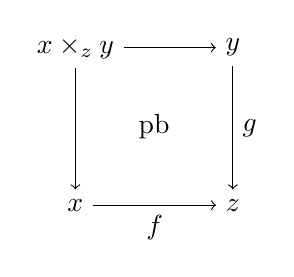
\begin{tikzpicture}
                    \node (X) at (0, -2) {$x$};
                    \node (Y) at (2, 0) {$y$};
                    \node (Z) at (2, -2) {$z$};
                    \node (pull) at (0, 0) {$x\times_zy$};
                    \node at (1, -1) {pb};
                    \draw[<-] (Z) -- node[below]{$f$} (X);
                    \draw[<-] (Z) -- node[right]{$g$} (Y);
                    \draw[->] (pull) -- (X);
                    \draw[->] (pull) -- (Y);
                \end{tikzpicture}
                \caption{Pullback square.}
                \label{fig:pullback_square}
            \end{subfigure}
            \begin{subfigure}[b]{0.49\textwidth}
                \centering
                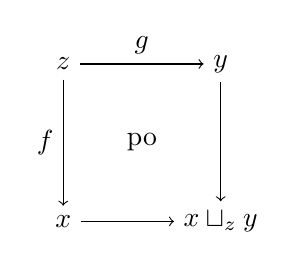
\begin{tikzpicture}
                    \node (X) at (0, -2) {$x$};
                    \node (Y) at (2, 0) {$y$};
                    \node (Z) at (0, 0) {$z$};
                    \node (push) at (2, -2) {$x\sqcup_zy$};
                    \node at (1, -1) {po};
                    \draw[->] (Z) -- node[left]{$f$} (X);
                    \draw[->] (Z) -- node[above]{$g$} (Y);
                    \draw[<-] (push) -- (X);
                    \draw[<-] (push) -- (Y);
                \end{tikzpicture}
                \caption{Pushout square.}
                \label{fig:pushout_square}
            \end{subfigure}
            \caption{Pullback and pushout diagrams.}
        \end{figure}
    \end{notation}

    \begin{example}[Product]\index{product}\index{fibre!product}
        If a terminal object $1$ exists, the pullback $x\times_1y$ is equal to the product $x\times y$.

        In fact, pullbacks are sometimes also called \textbf{fibred products}. The reason for this terminology is not only that products reduce to a particular case, but also that in the case of $\mathbf{Set}$ the pullbacks have a fibrewise product structure:
        \begin{gather}
            x\times_yz\cong\bigsqcup_{a\in x}f^{-1}(a)\times g^{-1}(a)\,.
        \end{gather}
    \end{example}
    \begin{example}[Kernel pair]\index{kernel}
        Consider a morphism $f:x\rightarrow y$. Its kernel pair is defined as the pullback of $f$ along itself.
    \end{example}

    \newdef{Pushout}{\index{pushout}\label{cat:pushout}
        The dual notion of a pullback, i.e.~the colimit of a span. See \cref{fig:pushout_square}.
    }

    \begin{property}
        Pullbacks preserve monos and pushouts preserve epis.
    \end{property}
    \newadef{Epimorphism}{\index{epimorphism}\label{cat:pushout_epi}
        A morphism whose cokernel pair is the identity.
    }

    \begin{property}[Pasting law]\index{pasting law}\label{cat:pasting_law}
        Consider a diagram of the form
        \begin{gather*}
            \begin{tikzpicture}
                \node (A) at (0, 0) {$A$};
                \node (B) at (2, 0) {$B$};
                \node (C) at (4, 0) {$C$};
                \node (X) at (0, -2) {$X$};
                \node (Y) at (2, -2) {$Y$};
                \node (Z) at (4, -2) {$Z$};
                \draw[->] (A) -- (B);
                \draw[->] (B) -- (C);
                \draw[->] (X) -- (Y);
                \draw[->] (Y) -- (Z);
                \draw[->] (A) -- (X);
                \draw[->] (B) -- (Y);
                \draw[->] (C) -- (Z);
            \end{tikzpicture}
        \end{gather*}
        If the right square is a pullback diagram, the left square is a pullback diagram if and only if the total diagram is. Dually, if the left square is a pushout diagram, the right square is a pushout diagram if and only if the total diagram is.
    \end{property}

    \begin{property}[\difficult{Span category}]\label{cat:span_category}
        Consider a category $\mathbf{C}$ with pullbacks. The category $\mathbf{Span}(\mathbf{C})$ is defined as the category with the same objects as $\mathbf{C}$ but with spans as morphisms. Composition of spans is given by pullbacks. By including morphisms of spans, $\mathbf{Span}(\mathbf{C})$ can be refined to a bicategory.
    \end{property}

    \newdef{Wedge}{\index{wedge}
        Consider a profunctor $\profunc{F}{C}{C}$. A wedge $e:w\rightarrow F$ is an object $w\in\ob{Set}$ together with a collection of morphisms $e_x:w\rightarrow F(x,x)$ indexed by $\mathbf{C}$ such that for every morphism $f:x\rightarrow y$ the following diagram commutes:
        \begin{gather*}
            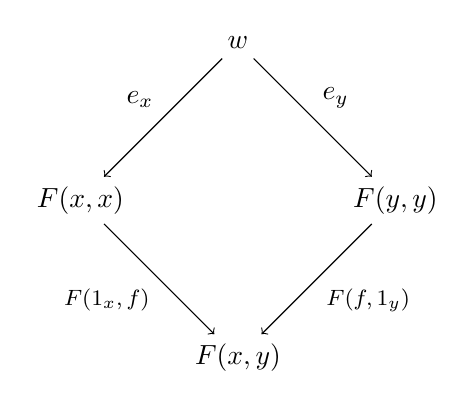
\begin{tikzpicture}
                \node (W) at (0, 4) {$w$};
                \node (F1) at (-2, 2) {$F(x,x)$};
                \node (F2) at (2, 2) {$F(y,y)$};
                \node (F) at (0, 0) {$F(x,y)$};
                \draw[->] (W) edge node[above left]{$e_x$} (F1) (F1) edge node[below left]{\footnotesize$F(\mathbbm{1}_x,f)$} (F);
                \draw[->] (W) edge node[above right]{$e_{y}$} (F2) (F2) edge node[below right]{\footnotesize$F(f,\mathbbm{1}_{y})$} (F);
            \end{tikzpicture}
        \end{gather*}
        As was the case for cones, this can be reformulated in terms of (di)natural transformations. A wedge $(w,e)$ of a profunctor $\profunc{F}{C}{C}$ is a dinatural transformation from the constant profunctor $\Delta_w$ to $F$.
    }
    \newdef{End}{\index{end}
        The end of a profunctor $\profunc{F}{C}{C}$ is defined as the universal wedge of $F$. The components of the wedge are called the \textbf{projection maps} of the end. This stems from the fact that for a discrete category the end coincides with the product $\prod_{x\in\ob{C}}F(x,x)$.

        This is equivalent to a definition in terms of equalizers. Consider the two canonical maps
        \begin{gather}
            \prod_{x\in\ob{C}}\mathbf{C}(x,x)\rightrightarrows\prod_{f:x\rightarrow y}\mathbf{C}(x,y)\,.
        \end{gather}
        This diagram can be interpreted as the product of all lower halves of the wedge diagrams above. It is not hard to see that its equalizer (universally) satisfies the wedge condition for all $f\in\mathrm{hom}(\mathbf{C})$.
    }
    \newnot{End}{
        The end of a profunctor $\profunc{F}{C}{C}$ is often denoted using an integral sign with subscript: \[\int_{x\in\mathbf{C}}F(x,x)\,.\] For the dual construction, called a \textbf{coend}, an integral sign with superscript is used.
    }
    \begin{example}[Natural transformations]\index{natural!transformation}
        Consider two functors $\func{F,G}{C}{D}$. The map $(x,y)\mapsto\mathbf{D}(Fx,Gy)$ gives a profunctor $\profunc{H}{C}{C}$. By looking at the wedge condition for this profunctor, the following equality for all morphisms $f:x\rightarrow y$ can be derived:
        \begin{gather}
            \tau_y\circ Ff = Gf\circ\tau_x\,,
        \end{gather}
        where $\tau$ is the wedge projection. Comparing this equality to \cref{cat:natural} gives
        \begin{gather}
            \label{cat:natural_end}
            \mathrm{Nat}(F,G) = \int_{x\in\mathbf{C}}\mathbf{D}(Fx,Gx)\,.
        \end{gather}
    \end{example}

    \begin{property}
        Using the continuity of the hom-functor (\cref{cat:continuity}), one can prove the following equality which can be used to turn ends into coends and vice versa:
        \begin{gather}
            \mathbf{Set}\left(\int^{x\in\mathbf{C}}F(x,x),y\right) = \int_{x\in\mathbf{C}}\mathbf{Set}\left(F(x,x),y\right)\,.
        \end{gather}
    \end{property}

    Using the above properties and definitions, one obtains the following two statements, called the \textbf{Yoneda reduction} and \textbf{co-Yoneda lemma}:
    \begin{property}[Ninja Yoneda lemma]\index{Yoneda!reduction}\index{co-!Yoneda|see{Yoneda, reduction}}\label{cat:ninja_yoneda}
        Let $\func{F}{C}{Set}$ be a covariant functor (similar statements hold for contravariant functors).
        \begin{align}
            &\int_{x\in\mathbf{C}}\mathbf{Set}\bigl(\mathbf{C}(-,x),Fx\bigr)\cong F\\
            &\int^{x\in\mathbf{C}}\mathbf{C}(x,-)\times Fx\cong F
        \end{align}
        For a generalization to the enriched setting see \cref{cat:enriched_ninja_yoneda}.
    \end{property}
    \begin{remark}
        A common remark at this point is the comparison with the Dirac distribution~\eqref{distribution:sieving_dirac_delta}:
        \begin{gather}
            \int \delta(x-y)f(x) = f(y)\,.
        \end{gather}
        By interpreting the functor $F$ as a function, the representable functors can be seen to behave as Dirac distributions.
    \end{remark}

    \begin{property}
        \begin{gather}
            \int_{F\in\mathbf{coPsh}(\mathbf{C})}\mathbf{Set}(Fx,Fy)\cong\mathbf{C}(x,y)
        \end{gather}
    \end{property}

    \newdef{Kan extension}{\index{Kan!extension}\label{cat:kan_extension}
        Consider two functors $\func{F}{A}{B}$ and $\func{G}{A}{C}$. The right Kan extension of $F$ along $G$ is given by the universal functor $\func{\mathrm{Ran}_GF}{C}{B}$ and natural transformation $\eta:\mathrm{Ran}_GF\circ G\Rightarrow F$:
        \begin{gather*}
            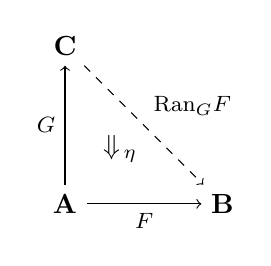
\begin{tikzpicture}
                \node (A) at (0, 0) {$\mathbf{A}$};
                \node (B) at (2, 0) {$\mathbf{B}$};
                \node (C) at (0, 2) {$\mathbf{C}$};
                \node at (0.7, 0.7) {$\Downarrow_{\,\eta}$};
                \draw[->] (A) -- node[left]{\footnotesize$G$} (C);
                \draw[->] (A) -- node[below]{\footnotesize$F$} (B);
                \draw[dashed, ->] (C) -- node[above right]{\footnotesize$\mathrm{Ran}_GF$} (B);
            \end{tikzpicture}
        \end{gather*}
        The left Kan extension $\mathrm{Lan}_GF$ is obtained by dualizing this construction.
    }

    \begin{property}[Complete categories]
        Complete (resp.~cocomplete) categories admit all right (resp.~left) Kan extensions.
    \end{property}

    \newdef{Preservation of Kan extension}{\label{cat:preservation_kan_extension}
        A Kan extension $\mathrm{Lan}_GF$ is said to be \textbf{absolute} if every functor with the same codomain as preserves the Kan extension, i.e.~a Kan extension is absolute if right whiskering it by another functor defines the Kan extension of the composition. If it is only preserved by all representable functors, the Kan extension is said to be \textbf{pointwise} or \textbf{strong}. Pointwise Kan extensions can be expressed as (co)limits, an expression is provided in \cref{cat:enriched_kan_extension} in the \textit{enriched setting} using (co)ends.
    }

    \newadef{Kan extension}{\label{cat:kan_extension_alternative}
        The definition above gives a natural isomorphism (here given for left extension):
        \begin{gather}
            \funccat{A}{B}(F,G^*-)\cong\funccat{C}{B}(\mathrm{Lan}_GF,-)\,.
        \end{gather}
        In the spirit of partial adjoints or partial limits, this construction defines so-called \textbf{local Kan extensions}. If local Kan extensions exist for all functors $F\in\funccat{A}{B}$, a right adjoint $\mathrm{Ran}_G:\funccat{A}{B}\rightarrow\funccat{C}{B}$ to the pullback functor $G^*:F\mapsto F\circ G$ is obtained. Similarly, left Kan extension can be defined as the left adjoint to the pullback functor.
    }
    \remark{Using this equivalence of hom-spaces, Kan extensions can be generalized from $\mathbf{Cat}$ to any \textit{2-category}.}

    \begin{example}[Limit]\index{limit}
        Denote the terminal category by $\mathbf{1}$. By choosing the functor $G$ in the definition of a right Kan extension to be the unique functor $!_{\mathbf{C}}:\mathbf{C}\rightarrow\mathbf{1}$, one obtain the universal property characterizing limits (\cref{cat:limit_uproperty}):
        \begin{gather}
            \lim F\cong\mathrm{Ran}_{!_C}F\,.
        \end{gather}
        Similarly, colimits can be obtained as left Kan extensions.
    \end{example}

    The existence of Kan extensions can also be used to determine the existence of adjoints.
    \begin{property}[Adjoint functors]
        A functor $\func{F}{C}{D}$ admits a left (resp.~right) adjoint if and only if the right (resp.~left) Kan extension of the identity functor $\mathbbm{1}_\mathbf{C}$ along $F$ exists. If it exists as an absolute extension, the left adjoint is given exactly by this Kan extension.
    \end{property}

    \newdef{Codensity monad}{\index{monad!codensity}\index{co-!dense}
        Consider a general functor $\func{F}{C}{D}$. If the right Kan extension $\mathrm{Ran}_FF$ exists, it defines a monad. Functors for which this monad is the identity are said to be \textbf{codense}.\footnote{Codense functors are usually defined in a different way, but one can show that this is an equivalent definition (hence the name).} Left Kan extensions give, by duality, rise to \textit{density comonads}.
    }

    \begin{property}[Faithfulness]
        Kan extension along a fully faithful functor is itself a fully faithful functor.
    \end{property}
    \begin{property}[Representability]
        (Left) Kan extension of a representable along a functor $F$ is equivalent to the representable of the image of $F$.
    \end{property}

    \begin{property}[Adjoint quadruple]\label{cat:kan_quadruple}
        Consider an adjunction $F\dashv G$ and consider Kan extension of presheaves taking values in a bicomplete category. In this case precomposition with (the opposite of) one of the adjoints coincides with Kan extension along (the opposite) of the other:
        \begin{align}
            (F^{\text{op}})^* &\cong \mathrm{Lan}_{G^{\text{op}}}\,,\\
            (G^{\text{op}})^* &\cong \mathrm{Ran}_{F^{\text{op}}}\,.
        \end{align}
        This implies that every adjunction induces an adjoint quadruple
        \begin{gather}
            \mathrm{Lan}_{F^{\text{op}}}\dashv\mathrm{Lan}_{G^{\text{op}}}\dashv\mathrm{Ran}_{F^{\text{op}}}\dashv\mathrm{Ran}_{G^{\text{op}}}\,.
        \end{gather}
    \end{property}

\section{Internal structures}\index{internal}\label{section:internal_category_theory}

    \begin{property}[Eckmann--Hilton argument]\index{Eckmann--Hilton!argument}\label{cat:eckmann_hilton}
        A monoid internal to $\mathbf{Mon}$, the category of monoids, is the same as a commutative monoid. (See also \cref{algebra:eckmann_hilton}.)
    \end{property}

    \newdef{Internal category}{\label{cat:internal_category}
        Let $\mathcal{E}$ be a category with pullbacks. A category $\mathbf{C}$ internal to $\mathcal{E}$ consists of the following data:
        \begin{itemize}
            \item an object $C_0\in\ob{\mathcal{E}}$ of objects;
            \item an object $C_1\in\ob{\mathcal{E}}$ of morphisms;
            \item source and target morphisms $s, t\in\mathcal{E}(C_1,C_0)$;
            \item an `identity-assigning' morphism $e\in\mathcal{E}(C_0, C_1)$ such that
            \begin{gather}
                s\circ e = \mathbbm{1}_{C_0}\qquad\qquad\qquad t\circ e = \mathbbm{1}_{C_0}\,;
            \end{gather}
            and
            \item a composition morphism $c:C_1\times_{C_0}C_1\rightarrow C_1$ such that the following equations hold:
            \begin{gather}
                \begin{aligned}
                    s\circ c = s\circ\pi_1\qquad\qquad&\qquad\qquad t\circ c = t\circ\pi_2\\
                    \pi_1 = c\circ(e\times_{C_0}\mathbbm{1})\qquad\qquad&\qquad\qquad c\circ(\mathbbm{1}\times_{C_0}e)=\pi_2\\
                    c\circ(c\times_{C_0}\mathbbm{1}) &= c\circ(\mathbbm{1}\times_{C_0}c)\,,
                \end{aligned}
            \end{gather}
            where $\pi_1,\pi_2$ are the canonical projections associated with the pullback $C_1\times_{C_0}C_1$ of $(s,t)$.
        \end{itemize}

        Morphisms between these categories, suitably called \textbf{internal functors}, are given by a pair of morphisms (in $\mathcal{E}$) between internal objects and morphisms, that preserve composition and identities. Internal natural transformations are defined in a similar way.
    }
    \begin{notation}
        The \textit{(bi)category} of internal categories in $\mathcal{E}$ is denoted by $\mathbf{Cat}(\mathcal{E})$. It should be noted that for $\mathcal{E}=\mathbf{Set}$, the ordinary category of small categories $\mathbf{Cat}(\mathbf{Set})=\mathbf{Cat}$ is obtained.
    \end{notation}
    \begin{adefinition}
        The above definition can be reformulated in a very elegant way. An internal category in $\mathcal{E}$ is a monad in the bicategory $\mathbf{Span}(\mathcal{E})$ as shown in \cref{fig:internal_cat_monad}.

        \begin{figure}[ht!]
            \centering
            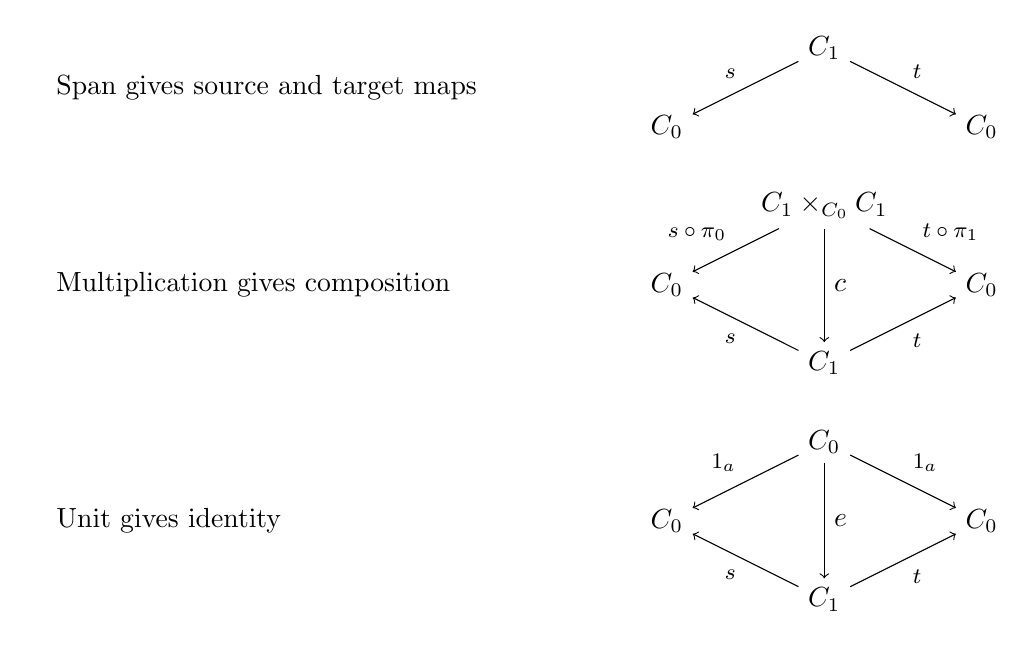
\begin{tikzpicture}
                \node[label={[align=left]right:Span gives source and target maps}] at (-10, -0.5) {};
                \node[label={[align=left]right:Multiplication gives composition}] at (-10, -3) {};
                \node[label={[align=left]right:Unit gives identity}] at (-10, -6) {};
                \node (mor) at (0, 0) {$C_1$};
                \node (ob1) at (-2, -1) {$C_0$};
                \node (ob2) at (2, -1) {$C_0$};
                \draw[->] (mor) -- node[above left]{\footnotesize$s$} (ob1);
                \draw[->] (mor) -- node[above right]{\footnotesize$t$} (ob2);
                \node (MM) at (0, -2) {$C_1\times_{C_0}C_1$};
                \node (M1) at (0, -4) {$C_1$};
                \node (O1) at (-2, -3) {$C_0$};
                \node (O2) at (2, -3) {$C_0$};
                \draw[->] (MM) -- node[above left]{\footnotesize$s\circ\pi_0$} (O1);
                \draw[->] (MM) -- node[above right]{\footnotesize$t\circ\pi_1$} (O2);
                \draw[->] (MM) -- node[right]{$c$} (M1);
                \draw[->] (M1) -- node[below left]{\footnotesize$s$} (O1);
                \draw[->] (M1) -- node[below right]{\footnotesize$t$} (O2);
                \node (O3) at (0, -5) {$C_0$};
                \node (M2) at (0, -7) {$C_1$};
                \node (O4) at (-2, -6) {$C_0$};
                \node (O5) at (2, -6) {$C_0$};
                \draw[->] (O3) -- node[above left]{\footnotesize$\mathbbm{1}_a$} (O4);
                \draw[->] (O3) -- node[above right]{\footnotesize$\mathbbm{1}_a$} (O5);
                \draw[->] (O3) -- node[right]{$e$} (M2);
                \draw[->] (M2) -- node[below left]{\footnotesize$s$} (O4);
                \draw[->] (M2) -- node[below right]{\footnotesize$t$} (O5);
            \end{tikzpicture}
            \caption{Internal category as a monad in $\mathbf{Span}(\mathcal{E})$.}
            \label{fig:internal_cat_monad}
        \end{figure}
    \end{adefinition}

    Functors between internal categories are not the only relevant morphisms. However, when defining (co)presheaves such as the hom-functor, a problem occurs. In $\mathbf{Cat}$ there exist, by definition, maps to the ambient category $\mathbf{Set}$ (ordinary category theory has a set-theoretic foundation). However, for internal categories there does not necessarily exist a morphism $\mathbf{C}\rightarrow\mathcal{E}$. To solve this problem, one can consider a more general structure.
    \newdef{Internal diagram}{\index{diagram}\label{cat:internal_diagram}
        A left module over a monad in $\mathbf{Span}(\mathcal{E})$. The dual notion is better known as an \textbf{internal presheaf}. The category of internal diagrams on an internal category $\mathbf{C}\in\mathbf{Cat}(\mathcal{E})$ is denoted by $\mathcal{E}^{\mathbf{C}}$.

        This can be spelled out more explicitly. An internal diagram in an internal category $\mathbf{C}\in\mathbf{Cat}(\mathcal{E})$ consists of:
        \begin{enumerate}
            \item a morphism $\gamma_0:F_0\rightarrow C_0$, and
            \item a morphism $\mathrm{ap}:F_0\times_{C_0}C_1\rightarrow F_0$
        \end{enumerate}
        satisfying:
        \begin{gather}
            \begin{aligned}
                \gamma_0\circ\mathrm{ap} &= d_1\circ\pi_{C_1}\\
                \mathrm{ap}\circ(\mathbbm{1}_{F_0}\times e)&=\pi_{F_0}\\
                \mathrm{ap}\circ(\mathrm{ap}\times\mathbbm{1}_{C_0})&=\mathrm{ap}\circ(\mathbbm{1}_{F_0}\times c)
            \end{aligned}
        \end{gather}
    }
    \newadef{Internal diagram}{
        An object of the slice category $\mathbf{Cat}(\mathcal{E})_{/\mathbf{C}}$ satisfying the following pullback condition:
        \begin{gather}
            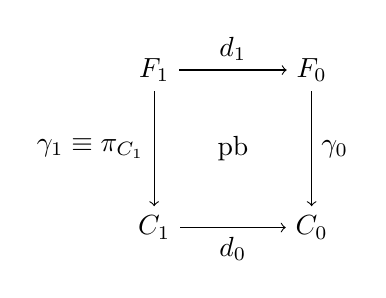
\begin{tikzpicture}[baseline=(current bounding box.center)]
                \node (F1) at (0, 0) {$F_1$};
                \node (C1) at (0, -2) {$C_1$};
                \node (F0) at (2, 0) {$F_0$};
                \node (C0) at (2, -2) {$C_0$};
                \node at (1, -1) {pb};
                \draw[->] (F1) -- node[left]{$\gamma_1\equiv\pi_{C_1}$} (C1);
                \draw[->] (F1) -- node[above]{$d_1$} (F0);
                \draw[->] (F0) -- node[right]{$\gamma_0$} (C0);
                \draw[->] (C1) -- node[below]{$d_0$} (C0);
            \end{tikzpicture}
        \end{gather}
    }

    In fact, this is a specific instance of an even more general concept. For more information on the definitions and applications, see~\citet{mac_lane_categories_2013, johnstone_topos_2014}.
    \newdef{Internal profunctor}{\index{pro-!functor}
        A bimodule between monads in $\mathbf{Span}(\mathcal{E})$. Together with the above definitions, this gives rise to an equivalence
        \begin{gather}
            \mathbf{Mod}(\mathbf{Span}(\mathcal{E}))\cong\mathbf{Prof}(\mathcal{E})\,.
        \end{gather}
    }

    \begin{construct}[Internal Yoneda profunctor]
        Consider an internal functor $\func{F}{C}{D}$. This functor induces two internal profunctors $\profunc{F_*}{D}{C}$ and $\profunc{F^*}{C}{D}$. For $F_*$ (the profunctor $F^*$ is defined similarly) the object span is defined as
        \begin{gather}
            C_0\overset{\pi_0}{\longleftarrow}C_0\times_{D_0} D_1\overset{t\circ\pi_1}{\longrightarrow}D_0\,.
        \end{gather}
        The action of $f\in D_1$ is given by postcomposition with $f$ in the second factor, while the action of $g\in C_1$ is given by precomposition with $Fg$ in the second factor and changing to the domain of $g$ in the first factor.

        It can easily be shown that the profunctors induced by an identity functor $\mathbbm{1}_{\mathbf{C}}$ have an object span that corresponds to the internal category $\mathbf{C}$ with the actions given by (internal) composition. In the case of $\mathcal{E}=\mathbf{Set}$, this boils down to the hom-functor. The fact that the object span is equivalent to the category $\mathbf{C}$ is essentially the Yoneda embedding. For this reason, this profunctor is in general called the (internal) Yoneda profunctor $\mathcal{Y}(\mathbf{C})$.
    \end{construct}

\subsection{Groupoids}\label{section:groupoids}

    \newdef{Groupoid}{\index{groupoid}\label{cat:groupoid}
        A (small) groupoid $\mathcal{G}$ is a (small) category in which all morphisms are invertible.
    }

    \begin{example}[Action groupoid]\index{groupoid!action}\label{cat:action_groupoid}
        Consider a set $X$ with an action of a group $G$. The action groupoid $X/\!\!/G$ is defined as the following category:
        \begin{enumerate}
            \item\textbf{Objects}: $X$,
            \item\textbf{Morphisms}: An arrow $x\rightarrow y$ for every $g\in G$ such that $g\cdot x=y$.
        \end{enumerate}
    \end{example}

    \begin{example}[Delooping]\index{delooping!of groups}\label{cat:group_delooping}
        Consider a group $G$. Its delooping $\mathbf{B}G$ is defined as the one-object groupoid for which $\mathbf{B}G(\ast,\ast)=G$.
    \end{example}
    \begin{property}[Representations]\label{cat:delooping_representation}
        Consider a group $G$ together with its delooping $\mathbf{B}G$. When considering \textit{representations} as functors $\rho:\mathbf{B}G\rightarrow\mathbf{FinVect}$, one can see that the intertwiners (\cref{group:equivariant}) are exactly the natural transformations. More generally, all $G$-sets (\cref{group:group_action}) can be obtained as functors $\mathbf{B}G\rightarrow\mathbf{Set}$.
    \end{property}

    \newdef{Core}{\index{core}\label{cat:core}
        Let $\mathbf{C}$ be a (small) category. The core $\mathrm{Core}(\mathbf{C})\in\mathbf{Grpd}$ of $\mathbf{C}$ is defined as the maximal subgroupoid of $\mathbf{C}$.
    }

    \newdef{Orbit}{\index{orbit}
        Let $\mathcal{G}$ be a groupoid with $O,M$ respectively the sets of objects and morphisms. On $O$ one can define an equivalence $x\sim y\iff\exists\phi:x\rightarrow y$. The equivalence classes are called orbits and the set of orbits is denoted by $O/M$.
    }
    \newdef{Transitive component}{\index{transitive!component}
        Let $\mathcal{G}$ be a groupoid with $O,M$ respectively the sets of objects and morphisms and let $s,t$ denote the source and target maps on $M$. Given an orbit $o\in O/M$, the transitive component of $M$ associated to $o$ is defined as $s^{-1}(o)$, or equivalently, as $t^{-1}(o)$.
    }
    \begin{property}
        Every groupoid is a (disjoint) union of its transitive components.
    \end{property}
    \newdef{Transitive groupoid}{\index{transitive!groupoid}
        A groupoid $\mathcal{G}$ is said to be transitive if for all objects $x\neq y\in\ob{\mathcal{G}}$, the set $\mathcal{G}(x,y)$ is not empty.
    }

\section{\difficult{Lawvere theories}}

    \newdef{Lawvere theory}{\index{Lawvere!theory}
        Let $\mathbf{F}$ denote the skeleton of $\mathbf{FinSet}$. A Lawvere theory consists of a small category $\mathbf{L}$ and a strict (finite) product-preserving \textit{identity-on-objects} functor $\mathcal{L}:\mathbf{F}^{\text{op}}\rightarrow\mathbf{L}$.

        Equivalently, a Lawvere theory is a small category $\mathbf{L}$ with a \textbf{generic object} $c_0$ such that every object $c\in\ob{L}$ is a finite power of $c_0$.
    }
    \begin{property}
        Lawvere theories $(\mathbf{L},\mathcal{L})$ form a category $\mathbf{Law}$. Morphisms between Lawvere theories are (finite) product-preserving functors.
    \end{property}

    \newdef{Model}{\index{model}\index{algebra}
        A model or \textbf{algebra} over a Lawvere theory $\mathbf{L}$ is a (finite) product-preserving functor $\func{A}{L}{Set}$.
    }

    \todo{COMPLETE}

\section{\difficult{Operad theory}}
\subsection{Operads}

    \newdef{Plain operad\footnotemark}{\index{operad}\index{arity}
        \footnotetext{Also called a \textbf{nonsymmetric operad} or \textbf{non-$\Sigma$ operad}.}
        Let $\mathcal{O}=\{P(n)\}_{n\in\mathbb{N}}$ be a collection of sets, called \textbf{$n$-ary operations} (where $n$ is called the \textbf{arity}). The collection $\mathcal{O}$ is called a plain operad if it satisfies following axioms:
        \begin{enumerate}
            \item $P(1)$ contains an identity element $\mathbbm{1}$.
            \item For all positive integers $n,k_1,\ldots,k_n$ there exists a composition map
            \begin{align}
                \circ&:P(n)\times P(k_1)\times\cdots\times P(k_n)\rightarrow P(k_1+\cdots+k_n)\nonumber\\
                &:(\psi,\theta_1,\ldots,\theta_n)\mapsto \psi\circ(\theta_1,\ldots,\theta_n)
            \end{align}
            that satisfies two additional axioms:
            \begin{itemize}
                \item\textbf{identity}:
                \begin{gather}
                    \theta\circ (\mathbbm{1},\ldots,\mathbbm{1}) = \mathbbm{1}\circ\theta = \theta,
                \end{gather}
                and
                \item\textbf{associativity}:
                \begin{align}
                    \psi\circ\Big(\theta_1\,\circ\,&(\theta_{1,1},\ldots,\theta_{1,k_1}),\ldots,\theta_n\circ(\theta_{n,1},\ldots,\theta_{n,k_n})\Big)\nonumber\\
                    &= \Big(\psi\circ(\theta_1,\ldots,\theta_n)\Big) \circ (\theta_{1,1},\ldots,\theta_{1,k_1},\theta_{2,1},\ldots,\theta_{n,k_n}).
                \end{align}
            \end{itemize}
        \end{enumerate}
        If the operad is represented using planar tree diagrams, the associativity obtains a nice intuitive form. When combining planar tree diagrams in three layers, the associativity axiom says that one can either first glue the first two layers together or one can first glue the last two layers together.
    }
    \remark{Plain operads can be defined in any monoidal category. In the same way symmetric operad can be defined in any symmetric monoidal category.}

    \begin{example}[Endomorphism operad]\index{endo-!morphism operad}
        Consider a vector space $V$. For every $n\in\mathbb{N}$, one can define the endomorphism algebra $\End(V^{\otimes n}, V)$. The endomorphism operad $\mathcal{E}\text{nd}(V)$ is defined as $\{\End(V^{\otimes n},V)\}_{n\in\mathbb{N}}$.
    \end{example}

    \newdef{$O$-algebra}{\index{algebra!over an operad}
        An object $X$ is called an algebra over an operad $O$ if there exist morphisms \[O(n)\times X^n\rightarrow X\] for every $n\in\mathbb{N}$ satisfying the usual composition and identity laws. Alternatively, this can be rephrased as the existence of a (plain) operad morphism $O(n)\rightarrow\mathcal{E}\text{nd}(X)$.
    }
    \begin{example}[Categorical $O$-algebra]
        An $O$-algebra in the category $\mathbf{Cat}$.
    \end{example}

\subsection{Algebraic topology}

    \newdef{Stasheff operad}{\index{Stasheff!operad}
        A topological operad $\mathcal{K}$ such that $\mathcal{K}(n)$ is given by the $n^{\text{th}}$ \textit{Stasheff polytope/associahedron}. Composition is given by the inclusion of faces.
    }
    \newdef{$A_\infty$-space}{\index{A${}_\infty$-space}\label{cat:A_infinity_space}
        An algebra over the Stasheff operad. This induces the structure of a multiplication that is associative up to a coherent homotopy.
    }

    \newdef{Little $k$-cubes operad}{\index{operad!little $k$-cubes}
        A topological operad for which every topological space $\mathcal{P}(n)$ consists of all possible configurations of $n$ embedded $k$-cubes in a (unit) $k$-cube. Composition is given by the obvious way of inserting one unit $k$-cube in one of the smaller embedded $k$-cubes.
    }
    \begin{property}[Recognition principle]\index{recognition principle}
        If a connected topological space $X$ forms an algebra over the little $k$-cubes operad, it is (weakly) homotopy equivalent to the $k$-fold loop space $\Omega^kY$ of another pointed topological space $Y$. For $k=1$, one should technically use the Stasheff operad, but it can be shown that this is related to the little interval operad.
    \end{property}

    @@ COMPLETE @@